\documentclass[
    PrintFilePath   = false,
    TwoSide         = false,
    StudentName     = 徐璨,
    StudentID       = 21020040058,
    AdvisorName     = 指导教师,
    Grade           = 2023,
    Major           = 统计学,
    Study           = 数理统计,          
    Supervisor      = 王伟刚,
    MajorType       = 统计学,
    Department      = 统计与数学学院,
    MajorFormat     = general,
    Degree          = graduate,   % 'undergraduate' or 'graduate'
    Type            = thesis,          % 'thesis'   or 'design'
    Period          = final,
    BlindReview     = false, 
    Language        = chinese,  
    GradLevel       = master, 
    Topic           = 研究方向, 
    ColaboratorName = 合作导师, 
    Title           = 用于创新药物设计的分子图扩散生成框架, 
]{zjuthesis}

\begin{document}

    \coverstyle
    % 切换封面
\ifthenelse{\equal{\BlindReview}{true}}
{
    % 盲审封面
\thispagestyle{cover}
\zihao{5}

\quad
% \begin{tabular}{l p{0.7\textwidth}}
%      \CheckedBox 全日制 & 非全日制
% \end{tabular}

\vskip 100pt 

\begin{center}
    \songti
    \bfseries
    \fontsize{30bp}{30bp}浙 \quad 江 \quad 省 \quad 硕 \quad 士 \quad 学 \quad 位 \quad 论 \quad 文
    
    \vskip 30pt 
    \fontsize{28bp}{28bp} 
    
\end{center}

\vskip 150pt
\begin{tabular}{l p{0.65\textwidth}}
\songti
\bfseries
    \textbf{\zihao{-2} 论文题目:} & \textbf{\zihao{-2} 用于创新药物设计的分子图扩散生成框架} 
\end{tabular}
\vskip 35pt
\begin{tabular}{l p{0.6\textwidth}}
\songti
\bfseries
    \textbf{\zihao{-2} 授予学位学科专业:统计学(理)} & \\
\end{tabular}
\vskip 35pt
\begin{tabular}{l p{0.5\textwidth}}
\songti
\bfseries
    \textbf{\zihao{-2} 学科专业代码:071400} & \textbf{\zihao{-2} } 
\end{tabular}
\vskip 35pt
\begin{tabular}{l p{0.4\textwidth}}
\songti
\bfseries
    \textbf{\zihao{-2} 研究方向:} & \textbf{\zihao{-2} 数理统计 } 
\end{tabular}
}
{
    %  中文封面
\thispagestyle{cover}
\begin{center}
    \zihao{-4} \songti
    \begin{tabularx}{\textwidth}{l l >{\raggedleft}X l}
        密级: \quad 公开 $\bigstar $ ~~ 2023年          &   &
        中图分类号:TP391& \quad\quad\quad \\
        \CheckedBox 全日制 ~~~ $\square$非全日制 & &
    \end{tabularx}
\end{center}

\vspace{10pt}

\begin{center}
    
\includegraphics[width=0.7\paperwidth]{figure/logo/zjgsuchar.png}
\end{center}

\vspace{10pt}

\begin{center}
    \textbf{
        \zihao{-0} \songti
        \TitleTypeNameCover
    }\\
    \vspace{10pt}
    % \textbf{\zihao{-1} \songti (专业学位)}
    
\end{center}

\ifthenelse{\equal{\DepartmentLines}{1}}
{
    %   DepartmentLines == 1
    \vskip 20pt
}
{
    %   DepartmentLines == 2
    \vskip 10pt
}

% \begin{center}
%     \includegraphics[width=0.15\paperwidth]{logo/zju.pdf}
% \end{center}

\ifthenelse{\equal{\DepartmentLines}{1}}
{
    %   DepartmentLines == 1
    \vskip 20pt
}
{
    %   DepartmentLines == 2
    \vskip 10pt
}

% Define multi line title



\begin{center}
    \bfseries
    \heiti
    \zihao{3}
    \begin{tabularx}{.8\textwidth}{l X<{\centering}}
        % If titles are too long for one row, please manually hardcode them in
        % multiple lines, as the english title example here.
        论文题目:&  \uline{\hfill  \heiti  基于图神经网络与对比学习 \hfill} \\
            ~   &   \uline{\hfill \heiti 的标签感知推荐算法研究 \hfill} \\
    \end{tabularx}
\end{center}

\vskip 60pt


\begin{center}
    \zihao{3}
    \kaishu
    \bfseries
    \renewcommand\arraystretch{1.1}	
    \begin{tabularx}{.8\textwidth}{l X<{\centering}}
        \textbf{作者姓名:} & \textbf{\uline{\hfill \StudentName 
 \hfill}} \\
        \textbf{学科专业:}   & \uline{\hfill \MajorType \hfill} \\
        \textbf{研究方向:}  &  \uline{\hfill \Study \hfill } \\
        \textbf{指导教师:}  &  \uline{\hfill \Supervisor \hfill} \\
    \end{tabularx}
\end{center}

\vskip 40pt

\begin{center}
    \zihao{-3} \bfseries
    \begin{tabularx}{.5\textwidth}{>{\zihao{3} \kaishu}l >{\zihao{3} \kaishu}X<{\centering}}
        \textbf{提交日期:} &  \textbf{2023年} \textbf{6月}
    \end{tabularx}
\end{center}

    \clearpage
    %  英文封面
\thispagestyle{cover}
% \vskip 50pt 
\begin{center}
    \textbf{\zihao{3} Dissertation Submitted to Zhejiang Gongshang University for Master's Degree of Engineering}
\end{center}

\vspace{40pt}

\begin{center}
    \zihao{3}
    A Diffusion-based Graph Generative Framework for {\itshape de novo} 3D molecule generation
\end{center}

\vspace{40pt}


\begin{center}
    \zihao{-3}
    \bfseries
    \renewcommand\arraystretch{1.1}	
    \begin{tabularx}{0.9\textwidth}{l X<{\centering}}
        \textbf{Author:} & \uline{\hfill Can Xu  \hfill} \\
        \textbf{Major:}   & \uline{ \hfill  Statistics \hfill} \\
        \textbf{Supervisor:}   &  \uline{ \hfill Prof. Weigang Wang \hfill} \\ 
    \end{tabularx}
\end{center}

\vspace{10pt}
\begin{center}
    
\includegraphics[width=0.2\paperwidth]{figures/zjgsu.png}
\end{center}
\vspace{10pt}
\begin{center}
    \textbf{
        \zihao{-3} 
        Dec. 2023}
\end{center}
\begin{center}
    \textbf{
        \zihao{-3} 
        School of Information and Electronic Engineering}
\end{center}

\begin{center}
\textbf{
        \zihao{-3} 
        Zhejiang Gongshang University
}
\end{center}
\begin{center}
    \textbf{
        \zihao{-3}
        Hangzhou,~310018,~P.R.~China
    }
\end{center}
}

    \prevstyle
    % Previous part
\cleardoublepage{}
\pagenumbering{Roman}
\thispagestyle{previous}
\pagestyle{previous}
\setcounter{page}{1}

\clearpage
\chapternonum{中文摘要}
% \begin{center}
%     \textbf{\heiti \zihao{3} \Title }
% \end{center}
\begin{center}
    \textbf{ \zihao{3} \heiti 摘\quad 要}
\end{center}
\songti \zihao{-4}
\linespreadonehalf

去噪扩散模型在多个研究领域显示出巨大潜力。现有的基于扩散生成模型在全新的三维药物分子设计任务中面临两个主要挑战。由于分子中的大部分重原子能够通过单键与多个原子相连,使用成对距离来建模分子几何结构是不足够的。因此,第一个挑战是提出一个有效的神经网络作为去噪核,能够捕捉复杂的原子间关系并学习高质量的特征。此外,由于图的离散性质,当前主流的基于扩散的药物分子设计模型严重依赖预设的规则,并以间接的方式生成边。故第二个挑战是将分子生成的过程与扩散的学习过程相结合,有效地准确预测键的存在。本文认为扩散过程中分子构象的迭代更新方式与分子动力学一致,故提出一种名为几何辅助的分子扩散(Geometric-facilitated Molecular Diffusion / GFMDiff)的新型药物分子设计框架。针对第一个挑战,我们引入了一种双轨Transformer网络(Dual-track Transformer Network / DTN),以全面挖掘全局空间关系并学习高质量的表示,从而提高对特征和几何结构的准确预测能力。至于第二个挑战,我们设计了几何辅助损失(Geometric-facilitated Loss / GFLoss),该损失在训练期间干预键的形成,而不是直接将边嵌入隐变量空间。本文在多个基准数据集上开展了全面实验表明GFMDiff性能达到该领域时下最优的水平。


\vspace{20pt}
\noindent \textbf{关键字:}扩散模型;分子生成;分子学习;图神经网络;几何神经网络

% 英文摘要
\clearpage
\addcontentsline{toc}{chapter}{英文摘要}
% \begin{center}
%     \zihao{3} \TitleEng
% \end{center}π
\begin{center}
    \textbf{\zihao{3} Abstract}
\end{center}
Denoising diffusion models have shown great potential in multiple research areas. Existing diffusion-based generative methods on {\itshape de novo} 3D molecule generation face two major challenge. Since majority heavy atoms in molecules allow connections to multiple atoms through single bonds, modeling molecule geometries using pair-wise distance is insufficient. Therefore, the first one involves proposing an effective neural network as the denoising kernel that is capable to capture complex interatomic relationships and learn high-quality features. Due to the discrete nature of graphs, mainstream diffusion-based methods for molecules heavily rely on predefined rules and generate edges in a indirect manner. The second one involves accommodating molecule generation to the learning process of diffusion and accurately predicting the existence of bonds effectively. In our research, we view the iterative way of updating molecule conformations in diffusion process is consistent with molecular dynamics and introduce a novel molecule generation method named Geometric-Facilitated Molecular Diffusion (GFMDiff). For the first challenge, we introduce a Dual-track Transformer Network (DTN) to fully excevate global spatial relationships and learn high quality representations which contribute to accurate predictions of features and geometries. As for the second challenge, we design Geometric-facilitated Loss (GFLoss) which intervenes the formation of bonds during the training period, instead of directly embedding edges into the latent space. Comprehensive experiments on current benchmarks demonstrate the superiority of GFMDiff.

\vspace{20pt}
\noindent \textbf{Keywords: Diffusion models; Molecule generation; Molecular learning; Graph neural networks; Geometry neural Networks}
\clearpage

% \cleardoublepage
% \addcontentsline{toc}{chapter}{目录}
\phantomsection
% \markloc
\tableofcontents

\begingroup
    \renewcommand*{\addvspace}[1]{}
    \cleardoublepage
    \phantomsection
    \marklof
    \listoffigures

    \cleardoublepage
    \phantomsection
    \marklot
    \listoftables
\endgroup



    \bodystyle
    \titlespacing{\chapter}{0pt}{-50pt}{0pt}
\zihao{-4}
\chapter{引言}
\label{chap:introduction}
\section{选题背景与研究意义}
\subsection{选题背景}
除图像、视频,音频与自然语言处理等领域,AI技术的快速发展也带动相关交叉学科的发展。AI4Science近年在计算生物、计算化学、材料设计、计算天文,计算育种等都有广泛应用,相关AI技术的应用能够大幅加速相关科学研究进展。在计算制药领域,近年来相关AI技术在药物性质预测,生成,开发,实验等领域的运用不仅加速相关研究的进展,也能够降低相关研究的研发成本。

基于AI的生成模型近十年来也被广泛研究,他们包括变分自编码器(Variational autoencoders / VAEs) \cite{vae_kingma_13},生成对抗模型(Generative adversarial networks / GANs) \cite{gan_goodfellow_14},流形模型(Normalizing flows / NFs) \cite{nice_dinh_15,density_dinh_17},自回归(Autoregressive models / ARs) \cite{ar_oord_16}与扩散模型(Diffusion) \cite{deepunsupervised_dickstein_15,generative_song_19}等。相关方法在图像,文字等方面也有了许多成功应用。

深度学习在分子化学领域近年来也有着成功的应用。以分子学习为例,化学分子常以简化分子线性输入规范字符串(Simplified molecular-input line-entry system / SMILES) \cite{smiles_weinberger_88}存储,每一个分子式对应一个SMILES字符串。随着早期深度学习方法,如卷积神经网络(Convolutional neural networks / CNNs) \cite{cnnsmiles_hirohara_18}和循环神经网络(Recurrent neural networks / RNNs) \cite{rnnsmiles_bjerrum_17,practicalmodel_liu_19,deeppurpose_huang_20}的发展,一些研究试图运用这些深度学习算法,对以字符串形式存在的分子式进行学习,以获得预测特定原子或是分子整体的性质的能力。随着图神经网络(Graph neural networks / GNNs) \cite{semisupervised_kipf_17,inductive_hamilton_17,howpowerful_xu_18}的出现,其对非结构化数据的建模能力和对节点间拓扑关系学习的能力被证明十分优异。分子作为自然界中天然存在的图结构,原子和键对应着图中的节点和边,这为分子学习提供了新的思路与方法。从最早的图卷积神经网络开始,相关研究者致力于提出新的图学习算法,以提升对分子图学习的性能。随着相关化学模拟技术的发展,让三维分子建模成为可能。这也在拓扑结构信息以外,提供了更丰富的几何构型信息,这也驱动着相关研究拓展至几何图神经网络上。分子三维构象允许研究者对分子进行更准确的研究,同时也推动更多复杂任务的出现,包括分子生成,Ligand生成,Protacs生成,药物亲和力预测,蛋白质预测等等。

\subsection{研究意义}
人工智能在智能计算相关研究中开始扮演越来越重要的角色,相关模型在药物发现、药物属性预测等应用中已经展现出良好的性能和极大的潜力。由于深度学习技术应用具备为药物研发的多阶段降本增效的潜力,在2022年,AI制药赛道相关企业融资总金额达百亿美元。在这一赛道竞逐的有国内互联网巨头如百度百图生科、华为EIHealth、腾讯云深智药,及初创企业晶泰科技,剂泰医药,星药科技等。相关成果已经展现出深度学习在该领域的强大性能和广阔前景。

\section{文献综述}
\subsection{基于深度学习的分子学习}
分子最早被表示为简化分子线性输入规范字符串,即SMILES字符串  \cite{smiles_weinberger_88},随着早期深度学习模型卷积神经网络和循环神经网络的发展,相关模型利用CNNs和RNNs对分子性质做出学习。Hirohara等 \cite{cnnsmiles_hirohara_18}的研究提出使用CNN对分子级别的特征和分子基团性质进行有效学习。由于RNNs在早期自然语言护理任务上有良好表现,Bjerrum \cite{rnnsmiles_bjerrum_17}提出LSTM-QSAR模型用于学习分子性质。

伴随图神经网络(GNNs)的发展,由于分子的形式天然的属于图结构,一些研究开始使用GNNs进行分子学习。CGCNN \cite{cgcnn_xie_18}将图卷积神经网络引入到分子性质学习,用以模拟并替代复杂的DFT计算。Xiong等 \cite{attentivefp_xiong_20}提出Attentive FP,一个结合注意力机制的图神经网络实现分子性质的有效学习与预测。GraSeq \cite{graseq_guo_20}提出在运用图神经网络学习拓扑结构同时,利用双向LSTM模型对SMILES分子式进行学习,通过两个通道联合预测分子性质。伴随相关技术的发展,研究者可以不再拘泥于原子拓扑结构,进而实现对分子三维结构的建模与学习。鉴于某一分子对应大量的同分异构体,而不同构象对应属性不尽相同,因此对三维构象的有效学习是十分必要的。EGNN \cite{egnn_satorras_21}在流行的图网络基础上,保留最基本的几何信息,即原子间距离,其简单的设计也成为了一些。在分子预训练框架GEM \cite{gem_fang_22}中,研究者提出GeoGNN图网络,将键长视作原子节点图的边特征,又对原子键构图,并将键角作为原子键图的边特征,通过在两个网络上的信息传递实现分子局部空间几何性质学习。Sch\"{u}tt等 \cite{schnet_schutt_17}在继承GNNs的信息传递范式的同时,将原子间距离用径向基函数(Radial basis funciton / RBF)建模后融入边特征,使算法对三维几何信息的有效学习的同时保证了等变性要求。SphereNet \cite{spherenet_liu_22}提出了基于球坐标系的信息传递范式SMP。通过一系列参考原子或键的规则,SMP在保证对原子对距离,键角和键扭转角这三个空间几何信息完整提取的同时,避免计算复杂度的爆炸式增长。ComENet \cite{comenet_wang_22}在ShpereNet的基础上,简化了空间几何信息的提取范式,在保证利用完整空间信息的前提下,以损失部分精度为代价,大幅度提升计算速度。

伴随着Transformer \cite{transformer_vaswani_17}相关研究在图像与文本领域的兴起,相关研究 \cite{smilestrans_honda_19,smilesbert_wang_19,chemberta_chithrananda_20}也利用Transformer对SMILES分子式进行学习。随着GTN \cite{gtn_yun_19}将Transformer引入图学习,越来越多的研究也将多头注意力机制用于分子图学习领域。大规模分子图预训练框架GROVER \cite{grover_rong_20}中,分子学习内核运用了GTransformer,同时学习分子中的原子与键的节点嵌入(embedding)或边嵌入。在分子预训练框架MPG \cite{mpg_li_21}中提出的图学习内核MolGNet放弃了对边嵌入的学习,仅利用多头注意力学习节点嵌入,结果证明了该图学习算法的有效性。

\subsection{基于深度生成模型的分子设计}
自深度学习研究兴起以来,深度生成模型一直是研究者重点研究的对象。作画、翻译、对话,渲染等应用能够直接服务于广大用户。主流的深度生成模型包括VAEs \cite{vae_kingma_13},GANs \cite{gan_goodfellow_14},NFs \cite{nice_dinh_15,density_dinh_17},ARs \cite{ar_oord_16}与Diffusion \cite{deepunsupervised_dickstein_15,generative_song_19}等。与图学习的演进过程相似,基于深度生成模型的分子设计也经历了从二维图结构到三维几何构象的演进。主流分子设计任务具体又可以被细分为:分子生成,分子优化,构象生成,蛋白质配体生成,蛋白质生成,蛋白降解靶向嵌合体生成。

分子生成的任务就是根据给定分子数据,使模型具备凭空生成全新且有效的药物分子图或三维结构。考虑到复杂药物分子主要由官能团等子结构组成,JT-VAE \cite{jtvae_jin_18}基于VAE生成树结构骨架,而后利用树结构骨架逐步生成分子图结构。GraphVAE \cite{graphvae_simonovsky_18}是早期的基于VAE的图生成研究,为避免离散化结构的线性表示的相关障碍,使其中解码器直接输出预设的最大概率的全连接图。基于NF模型,MoFlow \cite{moflow_zang_20}将隐式表征逐步映射到条件流过程中,模型首先生成连接原子的键,随后通过图条件流生成原子,并最终组成有效的分子图。

现有的基于扩散的分子生成模型较少,此领域最早的研究为EDM \cite{edm_hoogeboom_22},其基于EGNN \cite{egnn_satorras_21}的去噪过程内核,通过生成点云,再根据预设定的化学性质生成连接边的键。MDM \cite{mdm_huang_23}在此基础上,提出了全新的去噪内核,通过两个SchNet \cite{schnet_schutt_17}分别对局部节点和全局节点特征进行学习。由于这种扩散模型更擅长在连续样本空间上的学习,故主流方法并不直接预测分子图中边的存在性,针对这一问题,DiGress \cite{digress_vignac_22}和MiDi \cite{midi_vignac_23}提出将图邻接矩阵引入扩散过程,并相应将马尔可夫状态转移矩阵引入噪声序列而非传统的高斯噪声。GCDM \cite{gcdm_morehead_23}针对对空间几何信息提取不足的问题,引入ColfNet \cite{colfnet_du_22}相似的空间几何学习范式,实现了对几何信息的充分学习。

\subsection{扩散模型}
在图学习领域中,一个图可以被表示为一个元组 $\mathcal{G} = (\mathcal{V}, \mathcal{E})$,其中包含了一个节点集合 $\mathcal{V}$ 和一个边集合 $\mathcal{E}$。在训练阶段,模型学习图在扩散过程中的概率分布,并被用于后续的采样阶段,以迭代地方式生成新的图。基于扩散的生成模型因其在多个领域的生成任务中表现出色而受到广泛关注,例如计算机视觉 \cite{blendeddiffusion_avrahami_22,cascadeddiff_ho_22,gradforshapegen_cai_20,sgmpointcloud_luo_21},自然语言处理 \cite{struccddpm_austin_21,argmaxflow_hoogeboom_21,stepunrolled_savinov_22},以及其他各种跨学科任务等 \cite{cdvae_xie_22,housediffusion_shabani_23,nap_lei_23}。

人体骨架的表示形式与分子类似,都是表示为被边连接起的点云。不同之处在于生成人体骨架动作时,不需要对边的存在性进行预测。基于扩散模型,MoFusion \cite{mofusion_dabral_22}在人体动作生成中使用U-Net \cite{unet_ronneberger_15}作为扩散模型中去噪核心的架构。MoDi \cite{modi_raab_22} 利用结构感知神经滤波器和3D卷积,实现对每个关节的精确控制。

除了在分子生成和人体动作生成上的应用外,许多研究工作致力于将扩散过程用于其他形式的图数据生成。SaGess \cite{sagess_limnios_23}通过引入广义分治框架来增强DiGress \cite{digress_vignac_22}。对于2D图生成,EDP-GNN \cite{edpgnn_niu_20}将Score SDEs结合到离散图邻接矩阵生成中。在此基础上,GraphGDP \cite{graphgdp_huang_22}提出了名为Position-enhanced图得分网络的去噪核心,以实现对位置信息的进一步利用。GSDM \cite{gsdm_luo_22}不仅仅在边属性上进行采样,还利用了节点特征和图谱空间上的Score SDE高效地生成图,这在通用数据集和分子数据集上得到了验证。受VAEs启发,NVDiff \cite{nvdiff_chen_22}采用VGAE结构,首先对图在隐变量空间上的特征进行采样,然后将其解码为节点或边特征。SLD \cite{sld_yang_23}以类似的方式进行图生成任务。GraphARM \cite{ardiff_kong_23}通过引入节点吸收扩散过程,将自回归模型与扩散模型结合起来。EDGE \cite{edge_chen_23}将扩散模型引入大图生成,扩散过程中逐渐移除边,直到图为空。该模型还通过仅关注部分节点来避免生成过多的边。专为双曲图设计的HGDM \cite{hgdm_wen_23}在提取双曲嵌入的复杂几何特征方面表现出优良的性能。



\section{创新点}
近年来,深度生成模型,特别是基于扩散模型的生成模型 \cite{ddpm_ho_20,sgm_song_19,scoresde_song_21}在各个生成式人工智能研究领域中都取得了广泛且重大的进展。与生成方法的发展趋势相一致,分子发现领域的主流方法已经从之前的生成模型转变为基于扩散的模型,并从设计2D图形转变为3D构象。然而,3D分子生成面临两个主要挑战。第一个挑战是在预测准确稳定的分子构象方面,而另一个挑战则是充分利用几何信息以促进离散图结构的生成。在本文中,我们提出了几何促进的分子扩散(Geometric-facilitated Molecular Diffusion / GFMDiff),这是一种解决上述挑战的全新的3D分子生成方法。GFMDiff能够生成准确的3D几何构型,同时解决图自身离散性带来的诸多问题。

作为扩散模型中广泛采用的范式,去噪扩散概率模型(Denoising Diffusion Probabilistic Models / DDPMs) \cite{ddpm_ho_20,dpm_jascha_15}在各种生成任务中表现出色。通过在前向过程中逐渐添加高斯噪声,将输入数据转换为预定义的噪声分布,并在采样阶段迭代去噪,最终得到生成结果。与VAEs \cite{vae_kingma_13}和GANs \cite{gan_goodfellow_14}等端到端方法相比,这种在每个时间步训练扩散模型的方法在准确性、效率和训练难度方面表现更好。扩散模型在计算化学 \cite{edm_hoogeboom_22,targetdiff_guan_23}和生物学 \cite{diffab_luo_22,protseed_shi_23}等领域的应用已经显示出卓越的性能。在分子生成任务的背景下,逐步调整分子构象与分子动力学的核心原理高度一致。

全新的分子生成是分子生成领域一个重要的任务,该任务要求生成有效、新颖且结构稳定的分子。为了解决生成的3D构象所要求的等变性条件,一些基于扩散的方法 \cite{edm_hoogeboom_22,mdm_huang_23}通过原子间距离间接对分子进行建模,这直接反映了原子间相互作用力的强度。然而,早期的方法 \cite{edm_hoogeboom_22}没有解决多个原子之间的复杂原子间关系。而MDM \cite{mdm_huang_23}只是简单地使用阈值区分化学键和原子间力所造成的影响,而不考虑具体的原子和键的类型。最近的研究 \cite{moleformer_yuan_23}表明,键角之于分子学习与原子对间相互距离同样重要,但只有少数方法充分利用了空间信息。此外,由于分子扩散方法只作用于点云,传统的图卷积无法区分不同原子的重要性。鉴于这些挑战,我们设计了一种新颖的双轨分子学习框架,命名为双轨Transformer网络(Dual-track Transformer Network / DTN)。通过集成全局Transformer架构,本文将DTN作为扩散模型的去噪核函数,实现对空间几何信息的充分学习。

% 在分子生成领域,基于自回归模型(ARs)\cite{gschnet_wallach_19,gshperenet_luo_22}、正则化流(NFs)\cite{moflow_zang_20,graphaf_shi_20}、变分自编码器(VAEs)\cite{jtvae_jin_18,cgvae_liu_18}、能量模型(EBMs)\cite{graphebm_liu_21}等方法已经有了一些尝试。
鉴于扩散模型在连续数据上的出色性能,大多数分子图生成模型采用了在笛卡尔坐标和特征上采用扩散和去噪方法,然后基于预定义的规则生成分子图,而不是直接通过模型预测键的存在。间接生成图形的方式可能导致生成样本的稳定性和有效性有所下降。为了使扩散模型适用于分子的多模态数据,一些研究 \cite{edpgnn_niu_20,digress_vignac_22,midi_vignac_23}在扩散和去噪过程中引入了邻接矩阵。然而,将图和边嵌入模型中会导致计算成本的增加。在我们的研究中,我们将扩散模型视为一个过程,即在每个时间步根据局部多体原子间关系逐步更新原子信息。准确的特征学习有助于对分子构型进行精确预测。为了预测准确的分子构象,我们设计了一种在训练过程中减少嵌入和局部几何之间差距的方法。在本文中,我们通过精心设计的损失函数几何促进的损失函数(Geometric-facilitate Loss / GFLoss),在训练过程中积极的干预模型学习,促使模型生成稳定且合理的化学键。

在本文中,我们提出了用于3D分子生成的几何促进的分子扩散(Geometric-facilitated Molecular Diffusion / GFMDiff)框架。与先前的方法主要基于原子对距离学习原子特征不同,本文成功地将三元几何信息与原子对距离有效地结合到分子学习中。本领域大多数研究在生成式直接生成点云,并根据预设规则完成3D图结构的搭建。然而这种方法存在两个主要问题。首先,间接的图生成方式导致样本的稳定性和有效性下降。其次,传统的图卷积不足以区分局部和全局信息。为了解决第一个约束,本文设计了一个精巧的几何促进的损失函数(Geometric-facilitate Loss / GFLoss),在训练阶段主动引导键的形成。至于第二个约束,我们引入了双轨Transformer网络(Dual-track Transformer Network / DTN),这是一个基于全局Transformer的神经网络,以促进全面的几何学习和局部特征学习。最后在试验阶段,本文进一步在分子性质预测任务上检验了本文提出的DTN神经网络的有效性。总而言之,本文的创新点如下:
\begin{itemize}
    \item 本文提出的GFMDiff框架及其中的DTN网络,能够综合且全面的利用空间信息,以捕捉原子之间的多体相互作用,这对生成有效且稳定的全新分子至关重要。
    \item 为了解决图形的离散性问题,引入了一个精心设计的GFLoss,以促进键的形成,高效的处理由图内在离散性与扩散模型不兼容带来的挑战。
    \item 提出了DTN作为全局图卷积的替代方案,可以有效地捕捉全局和局部信息,并在后续的分子性质预测任务中进一步验证其有效性。
\end{itemize}

\section{基本框架}
本文可分为四章,每章的主要内容如下:

第一章为引言,本文在该部分介绍了分子生成的研究背景及意义,相关研究领域的研究现状及本文的主要创新点。

第二章中,本文在该部分介绍了分子图学习,等变性要求和基于扩散的生成模型等预备知识。

第三章中,本文在该部分介绍了本文提出的GFMDiff框架,包括其中的DTN去噪内核,GFLoss损失函数及相关训练过程。

第四章中,本文在该部分介绍了本文的GFMDiff模型在多个分子生成任务中的表现及其中去噪核心DTN在多个分子学习任务上的表现。

第五章中,本文在该部分总结了本文研究的内容,并对未来发展做出展望。

    \chapter{分子图学习与基于扩散模型的图生成}
\label{chap:diffusion-based_molgen}

\section{分子图学习}
在图学习中通常有两类监督任务:节点分类/回归和图分类/回归。对于图学习,一个分子可以被抽象为一个图 $\mathcal{G} = (\mathcal{V}, \mathcal{E})$,其中 $|\mathcal{V}| = n$表示节点(原子)的集合,$|\mathcal{E}| = m$ 表示分子中的边(化学键)的集合。我们用$e_i$表示节点 $i$的特征,用$e_{ij}$表示边$(i, j)$的特征。

在节点分类或回归任务中,每个节点$i$都有一个标签或目标$y_i$。任务目标是通过学习,预测未见节点的标签。这个任务可被应用于许多应用,比如识别分子中的功能团或预测各个原子的性质。

此外,在图分类或回归任务中,给定一组图$\{ \mathcal{G}_1, \mathcal{G}_2, ..., \mathcal{G}_N \}$和对应的标签或目标 $\{ y_1, ..., y_N \}$。此时任务目标是根据图的结构和节点边的特征,预测给定图的标签或目标。这个任务被广泛应用于化合物分类或基于结构预测分子性质等。

在这两类任务中,目标是利用监督学习技术训练模型,有效地捕捉图的结构与相关标签/目标之间的关系。现有的图学习方法主要有基于图神经网络的模型和基于Transformer架构的模型。

图神经网络(Graph Neural Networks / GNNs),近来在知识图谱、社交网络和药物发现等各个领域引起了广泛的关注。GNNs的核心操作在于将图中节点或边之间的特征进行传递(也称为邻居聚合)。消息传递操作通过聚合节点$i$的邻居节点和边的隐式特征来迭代更新节点$i$自身的隐式特征$e_i$。一般来说,消息传递过程包含多轮迭代,每轮迭代可以被视为对更远距离邻居的消息聚合。假设有$L$轮迭代,第$l$轮迭代会将目标节点的l跳邻居特征注入目标节点的隐式特征。第$l$轮迭代中,消息的传递与聚合可被表示为:
\begin{eqnarray}
    &m_j^{(l)} = {\rm MSG}^{(l)}(e_j^{(l-1)}), \ j \in \mathcal{N}_i, & \\
    &e_i^{(l)} = {\rm AGG}^{(l)}(\{ m_j^{(l)}, \ j \in \mathcal{N}_i \}, \ m_i^{(l)} ), &
\end{eqnarray}
其中$m_j^{(l)}$为聚合后的消息,MSG为消息聚合函数,主流的选择包括多层感知机(MLP),可学习权重。$e_i^{(l)}$为聚合后的目标节点特征,AGG为聚合函数,主流的方式有平均值池化、最大池化和图注意力机制等。对每一次消息传递,MSG和AGG函数都可能存在可训练的参数,这些参数在每轮迭代中一般是共享的。经过$L$次消息传递与聚合后,最后一次迭代后的隐式特征被视为模型预测的节点嵌入,即$e_i^{(L)}$。最后,根据具体任务需要,运用相应的READOUT函数即可得到节点信息或是全图级别的信息。

近年来,伴随Transformer模型的出现,一些研究也开始将该架构引入图学习中。多头注意机制是Transformer的核心模块,它将多个注意力层堆叠在一起,实现并行运算。一个注意力层的核心要素一般为一组查询、键、值组成,记为$(\mathbf{Q}, \mathbf{K}, \mathbf{V})$。通过查询和键的点积,经过softmax函数归一化后即可获得注意力概率,具体可表示为:
\begin{eqnarray}
    {\rm Attention}(\mathbf{Q}, \mathbf{K}, \mathbf{V}) = {\rm softmax}(\frac{\mathbf{Q} \cdot \mathbf{K}^T}{\sqrt{d}}) \cdot \mathbf{V},
\end{eqnarray}
其中$d$为注意力头数。多头注意力机制已经在广泛的应用中证明了其优异的性能。在图学习领域,基于多头注意力机制的Transformer机制不依赖于图神经网络在每一层之间进行消息传递的范式,能够对全局信息有更全面的建模。但是相应的,与图神经网络相比,Transformer模型对算力也有更高的要求。

\section{等变性要求}
等变性是涉及到几何空间的深度学习模型需要满足的基础条件。设$T_g: X \to X$是在$g \in G$上对$X$的变换集合。我们称一个函数$\phi: X \to Y$在$g$上具有等变性,如果存在一个变换$S_g: Y \to Y$,使得下式成立:
\begin{equation}
    \phi (T_g(x)) = S_g(\phi (x))
\end{equation}

假设$\phi (\cdot)$是一个非线性函数,$x = (x_1, ..., x_N) \in \mathbb{R}^{N \times d}$是在$d$维空间中的点云输入集合,$\phi (x) = y \in \mathbb{R}^{N \times d}$是经变换后的点云集合,$T_g (x) = x + g$和$S_g(y) = y + g$分别是针对输入集合和输出集合的平移变换,如果两个变化具备等变性,那么输入和和输出也是等变的。如果变换 $\phi : X \to Y$对平移变换具有等变性,则先对输入集合进行平移$T_g(x)$,然后对其应用函数$\phi(T_g(x))$,得到的结果与先对原函数进行变换得到$y = \phi(x)$,然后对输出进行等效平移$T_g(y)$ 后的结果相同,满足方程$\phi (x+g) = \phi (x) + g$。在本工作中,我们探讨了以下三种粒子集合等变性:
\begin{itemize}
    \item 1. 平移等变性:将输入集合在$g \in \mathbb{R}^d$上进行平移,结果等价于对输出进行平移。令该变换$x + g$表示为$(x_1+g, ..., x_N + g)$,则有 $y+g = \phi (x+g)$。
    \item 2. 旋转和反射等变性:对于任意正交矩阵$Q \in \mathbb{R}^{d \times d}$,对输入做旋转或反射变化等价于对输出结果做旋转或反射变化$Qy = \phi(Qx)$。
    \item 3. 置换等变性:对输入进行置换会等效地对输出进行相同的置换。$P(y) = \phi(P(x))$,其中$P$是行索引上的一种置换。
\end{itemize}
等变性要求在高维空间内的深度学习中是一项需要满足的基本条件。对于在$n$维空间上同时满足平移,旋转,和置换不变性的变换集合,可记为E(n)。


\section{基于扩散模型的图生成}
扩散模型在生成模型中引起了相当大的关注。通过学习逆过程的去噪核,这些模型能够揭示噪声样本的潜在分布。在给定一段数据的情况下,正向过程被视为马尔可夫链,通过学习可学习参数控制噪声强度,逐渐向数据添加高斯噪声$T$次。在生成过程中,模型将噪声还原回真实数据的原始分布。

\subsection{扩散过程}
设$G_t (t=0, 1, ..., T)$表示分子几何信息的分布,$\beta_t \in (0, 1), t=0, 1, ..., T$表示马尔可夫链的噪声方差序列。因此我们可以得到几何信息在$t$或$T$时刻在后验分布:
\begin{eqnarray}
&q(G_{1:T} | G_0) = \prod^T_{t=1} q(G_t | G_{t-1}), & \\
&q(G_t | G_{t-1}) = \mathcal{N}(G_t; \sqrt{1-\beta_t}G_{t-1}, \beta_t I).&
\end{eqnarray}

随着时间步$t$的增加,扩散过程逐步将更多的噪声添加到原始数据分布,具体表现为噪声方差$\beta_t$从0平滑地过渡到1。设$\bar{\alpha}_t = \prod^t_{s=1} \alpha_s = \prod^t_{s=1}(1-\beta_s)$,则任意$t$时刻样本数据的分布可以表示为:
\begin{equation}
    q(G_t|G_0) = \mathcal{N}(G_t; \sqrt{\bar{\alpha}_t} G_0, (1 - \bar{\alpha}_t) I).
\end{equation} 
经过足够多的时间步$T$,初始分布被转化成白噪声,即$G_t \sim \mathcal{N}(G_t; 0, I)$。在此基础上,去噪过程会将白噪声反向还原成不带噪声的样本分布。

\subsubsection{去噪过程}
在去噪过程(也称采样过程)中,模型通过学习接近真实的逆过程$q(G_{t-1} | G_t)$的马尔可夫核函数$p_\theta(G_{0:T-1}| G_{T}) = \prod^T_{t=1} p_\theta(G_{t-1} | G_t)$来重新构建原始的几何信息。每个时间步中学习到的去噪分布为: 
\begin{equation}
  p_\theta(G_{t-1} | G_t) = \mathcal{N}(G_{t-1}; \mu_\theta(G_t, t), \sigma_t^2 I),
\end{equation}
其中$\mu_\theta(G_t, t)$是可训练的神经网络,被用于近似估计均值,$\sigma^2_t = \frac{(\beta_t - \beta_{t-1})\beta_{t-1}}{(1 - \beta_{t-1}) \beta_t}$是预定义的方差。在采样过程开始时,$p_\theta(G_T)$采样自标准高斯分布中,然后通过迭代的去噪过程逐步优化参数化的神经网络,并最终还原得到初始时刻的几何信息,即采样结果。

理论上,神经网络的目标函数采用数据的对数似然函数的变分下界形式:
\begin{eqnarray}
    &{\rm log}p(G) \geq \mathcal{L}_{base} + \sum_{t=0}^T \mathcal{L}_t,& \\
    &\mathcal{L}_{base} = -KL(q(G_T|G_0)|p(G_T)),& \\
    &\mathcal{L}_t = KL(q(G_{t-1}|G_t)|p(G_{t-1}|G_t)). &
\end{eqnarray}
然而,研究发现,神经网路预测的高斯噪声$\epsilon$能够更容易的用于训练。因此,在实际优化神经网络时,神经网路常用的目标函数$\mathcal{L}_t$ \cite{vaediff_kingma_21}形式为:
\begin{equation}
    \mathcal{L}_t = E_{\epsilon_t \sim \mathcal{N}(0, I)}[\frac{1}{2}(1- \frac{{\rm SNR}(t-1)}{{\rm SNR}(t)})||\epsilon_t - \hat{\epsilon}_t||^2].
\end{equation}



    \chapter{几何促进的3D分子图生成(GFMDiff)}
\label{chap:gfmdiff}

在本节中,本文将着重介绍创新3D药物分子设计的模型框架,具体包括本文提出的E(n)等变去噪内核,几何信息促进的损失函数,扩散及去噪过程和优化目标。本文提出的创新3D药物分子设计整体框架GFMDiff由图~\ref{fig:gfmdiff}~所示。

\begin{figure}[h]
    \centering
    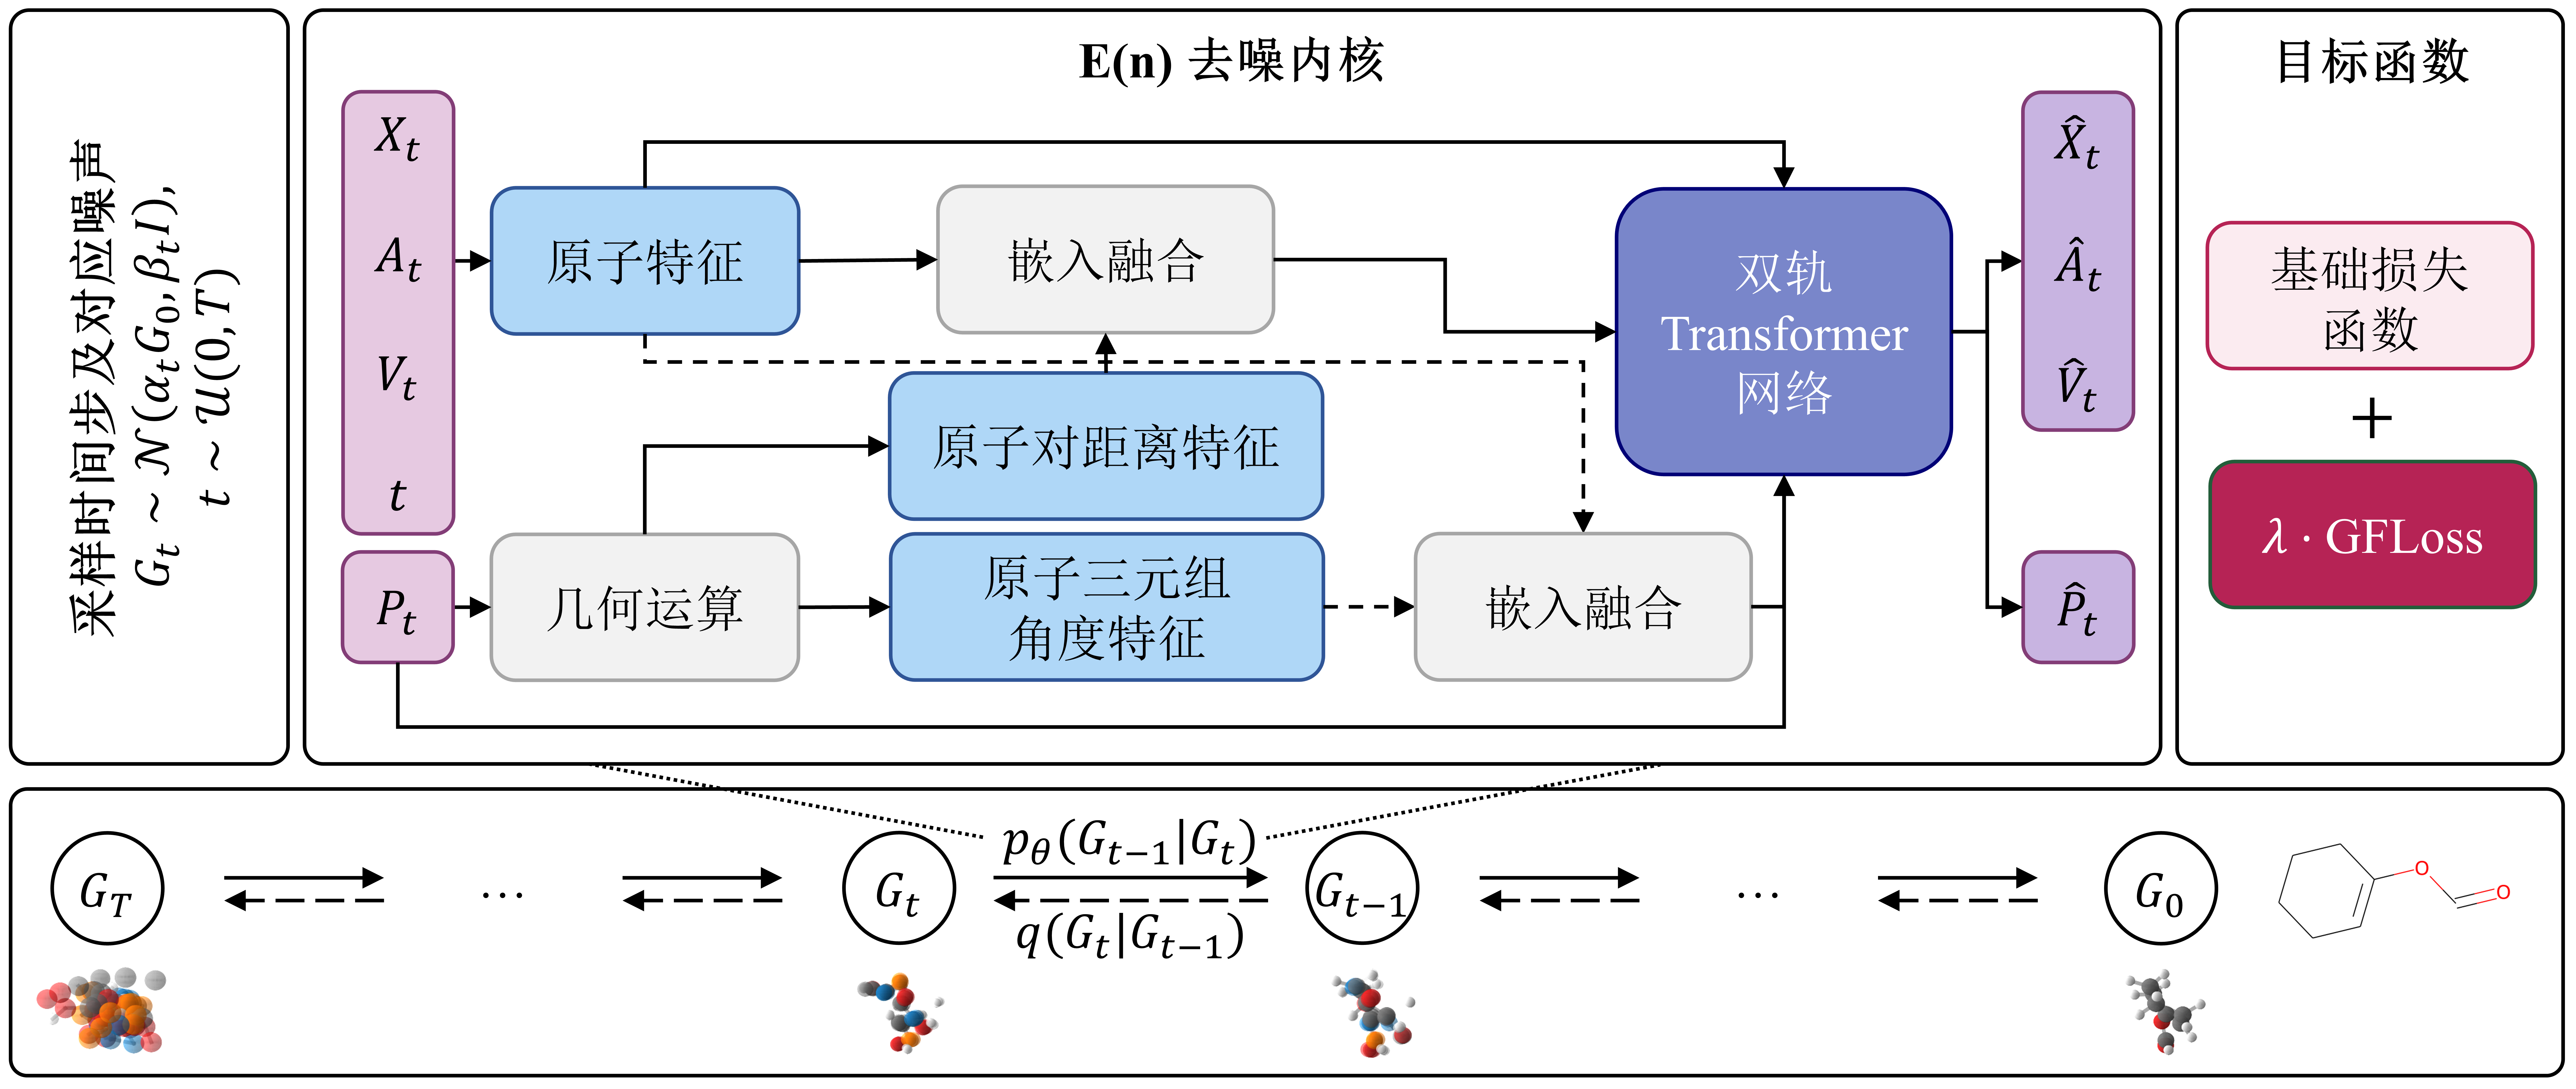
\includegraphics[width=\linewidth]{figures/overview_gfmdiff.png}
    \caption{GFMDiff模型框架示意图}
    \label{fig:gfmdiff}
\end{figure} 

对于每个训练样本,模型的输入为随机选取的时间步$t$和采样自对应时刻噪声分布的样本。通过几何计算及编码,得到的原子特征,原子对距离特征,三元组角度特征将被用于E(n)等变的去噪内核DTN中的分子学习,并得到更新后的样本在$t-1$时刻的分布,即对应的原子特征和位置信息。

\section{双轨Transformer网络(DTN)}
在这个小节中,我们将详细介绍作为GFMDiff的E(n)等变去噪内核的双轨Transformer网络(Dual-track Transformer Network / DTN)。DTN被设计用于有效捕捉原子之间的关系和原子特征。由于三维分子几何具有旋转、平移、反射和排列等不变性质,使得去噪核满足这些性质是很重要的。本文所提出的DTN不仅是E(n)等变的,还能充分利用空间信息,进而预测高质量的原子及分子特征。图~\ref{fig:dtn}~为DTN的模型结构。

\begin{figure}[h]
  \centering
  
\includegraphics[width=\linewidth]{figures/structure_dtn.png}
  \caption{DTN去噪内核结构示意图}
  \label{fig:dtn}
\end{figure}

% 传统的图神经网络用于学习图结构数据的拓扑信息,仅仅是置换等变的。尽管已经有许多努力致力于赋予GNN上述性质,我们提供了另一种解决这个问题的视角。

在我们提出的方法中,我们将具有总原子数$N$的输入分子视为$G = (P, X, A, V)$,其中$P = (p_1, p_2, ..., p_N) \in \mathbb{R}^{N \times 3}$表示原子坐标,$X = (x_1, x_2, ..., x_N) \in \mathbb{R}^{N \times nf}$表示原子编号的独热编码,$A = (a_1, a_2, ..., a_N) \in \mathbb{R}^{N}$表示原子编号,$V = (v_1, v_2, ..., v_N) \in \mathbb{R}^{N}$表示原子化合价数。为了确保等变性,DTN利用原子对距离信息和三元组角度信息捕捉几何信息。原子$i$和$j$之间的欧几里得距离反映了原子间相互作用的强度,可以通过以下公式获得:
\begin{equation}
    d_{ij} = ||p_i - p_j||_2.
\end{equation}
在分子中,除了氢原子,其他多数原子能够形成超过一个单键,故存在大量原子间的多体复杂关系。因此仅使用原子对距离是不足以充分提取空间几何信息。本文提出进一步使用以下公式计算原子三元组间的夹角:
\begin{equation}
    \varphi_{ijk} = \arccos \left(\frac{(p_i - p_j) \times (p_i - p_k)}{||p_i - p_j||_2 \times ||p_i - p_k||_2} \right). 
\end{equation}
经过上述几何计算,本文通过径向基神经网络(Radial Basis Function / RBF)编码得到可以被用作神经网络学习的原子对距离特征和三元组角度特征:
\begin{eqnarray}
    &e_{ij} = {\rm Linear}({\rm RBF}(d_{ij}), e_i, e_j),& \\
    &e_{ijk} = {\rm Linear}({\rm RBF}(\varphi_{ijk}), e_i, e_j, e_k),&
\end{eqnarray}
其中$e_i = {\rm Embedding}(x_i, a_i, v_i)$是原子$i$的节点嵌入,由原子序数和化合价决定。这些特征随后被输入到$L$层的DTN中。RBF函数是一种常用的径向基函数。在机器学习和模式识别领域中,RBF函数常用于对数据进行特征编码和表征,以距离特征计算为例:
\begin{eqnarray}
    &K(d_{ij}, \mu_k) = {\rm exp} \left(- \frac{||d_{ij} - \mu_k||^2}{2\sigma^2}\right), & \\
    &{\rm RBF}(d_ij) = {\rm Linear}(K(d_{ij}, \mu_k)), &
\end{eqnarray}
其中中心$\mu_k$和自由参数$\sigma$为RBF函数参数。在距离特征计算时,$\mu$满足$0 \text{\AA} \leq \mu_k \leq 10 \text{\AA}$并以$0.2\text{\AA}$的间隔切片,$\sigma$满足$\frac{1}{2\sigma^2} = 10 \text{\AA}$。经过切片操作后,$K(d_{ij}, \mu_k)$的维度为50,故需要通过线性层将RBF特征映射到与原子对特征维度一致的高位特征空间内。在角度计算时,$\mu$满足$0 \text{\AA} \leq \mu_k \leq \pi \text{\AA}$并以$0.1\text{\AA}$的间隔切片,$\sigma$满足$\frac{1}{2\sigma^2} = 10 \text{\AA}$。

DTN的每一层由以下组件组成:原子-原子对轨道、原子对-三元组轨道和连接模块。原子-原子对轨道模拟了原子之间的相互作用力对目标原子的影响,而原子对-三元组轨道则模拟了键角对边潜在的影响。连接模块作为两个轨道之间的桥梁,将原子特征注入到原子对特征中,以促进更好的表示学习。

原子-原子对轨道预测其他原子和原子之间相互作用力对目标原子的影响。该轨道将原子嵌入$e_i$和原子对嵌入$e_{ij}$作为输入,其中用于更新原子特征的多头注意力机制模块为:
\begin{eqnarray}
    &e_i = {\rm LayerNorm}(e_i),& \\
    &e_{ij} = {\rm LayerNorm}(e_{ij}),& \\
    &\mathbf{Q}_i = {\rm Linear}(e_i),& \\ 
    &\mathbf{K}_i = {\rm Linear}(e_i) + {\rm Linear}(e_{ij}),& \\
    &a_i = {\rm Dropout} \left({\rm softmax} \frac{\mathbf{Q}_i \mathbf{K}_i^T}{\sqrt{d_h}} \right), & \\
    &\mathbf{V}_i = {\rm Linear}(e_{ij}) + {\rm Linear}(e_{i}) + {\rm Linear}(e_{j}),& \\
    &\hat{e}_i = {\rm Linear}(a_i \mathbf{V}_i^T),&
\end{eqnarray}
其中$d_h$是多头注意力机制的头的数量。原子嵌入首先通过原子-原子对轨道输出的原子嵌入相加的方式更新,然后通过给前馈网络。在每一层DTN中,原子会接收来自于其他原子和相应的原子对的信息。

类似地,原子对-三元组轨道预测了复杂几何亚结构对原子间相互作用力的影响。其中的多头注意力机制模块可以表示为:
\begin{eqnarray}
    &e_{ij} = {\rm LayerNorm}(e_{ij}),&\\
    &e_{ijk} = {\rm LayerNorm}(e_{ijk}),&\\
    &\mathbf{Q}_{ij} = {\rm Linear}(e_{ij}),& \\ 
    &\mathbf{K}_{ij} = {\rm Linear}(e_{ij}) + {\rm Linear}(e_{ijk}),& \\
    &a_{ij}= {\rm Dropout} \left({\rm softmax} \frac{\mathbf{Q}_{ij} \mathbf{K}_{ij}^T}{\sqrt{d_h}} \right), & \\
    &\mathbf{V}_{ij} = {\rm Linear}(e_{ij}) + {\rm Linear}(e_{ijk}),& \\
    &\hat{e}_{ij} = {\rm Linear}(a_{ij} \mathbf{V}_{ij}^T).&
\end{eqnarray}
值得注意的是,三元组嵌入$e_{ijk}$在Transformer结构中不会得到更新,因为这会显著增加计算资源的需求。它们只会在原子坐标更新时利用特征编码得到更新。

连接模块的作用是将原子嵌入融合到原子对嵌入中。对于原子对嵌入$e_{ij}$,它同时接收来自连接模块的原子特征信息和来自原子对-三元组轨道的局部空间信息。
\begin{equation}
    e_{ij} = {\rm LayerNorm}(e_{ij} + {\rm Linear}({\rm Linear}(e_i) \otimes {\rm Linear}(e_j)))
\end{equation}

在更新坐标的方法上,我们遵循EDM \cite{edm_hoogeboom_22}和MDM \cite{mdm_huang_23}中的相关设计。
\begin{equation}
    \hat{p}_i = p_i + \sum_{j \neq i} \frac{p_i - p_j}{d_{ij} + 1} {\rm Linear}(\hat{e}_i, \hat{e}_j, d_{ij}^2, \hat{e}_{ij})
\end{equation}

由于在该坐标更新模块中,仅依赖于原子间相对距离更新原子坐标,故其严格遵循E(n)等变性要求。在原子坐标得到更新后,原子对和原子三元组的嵌入也将得到更新:
\begin{eqnarray}
  &e_{ij} = {\rm Linear}[{\rm Linear}({\rm RBF}(\hat{d}_{ij}), \hat{e}_{ij}), \hat{e}_i, \hat{e_j}],& \\
  &e_{ijk} = {\rm Linear}({\rm RBF}(\hat{\varphi}_{ijk}), e_{ijk}). &
\end{eqnarray}

更新后的原子对距离特征和三元组角度特征可以被用作下一层DTN网络的输入,或是直接作为去噪内核的输出。运用该种方法能够避免通过神经网络直接更新三元组嵌入,故而在极大减小计算需求的同时,又能通过简单的线性层更新能够反映几何特征的三元组特征。在算法~\ref{alg:dtn}~中详细的介绍了每一层的DTN的计算流程。

\begin{algorithm}[H]
    \caption{DTN去噪内核伪代码}
    \label{alg:dtn}
    \begin{algorithmic}
    \STATE {\bfseries Input} 原子特征$e_i$,原子对特征$e_{ij}$,三元组特征分子$e_{ijk}$和几何坐标$p_t$;
    \STATE 层归一化$e_i$和$e_{ij}$;
    \STATE 计算多头注意力概率$a_i$和值$\mathbf{V}_i$;
    \STATE 得到更新的原子特征残差$\hat{e}_i$并更新原子特征$e_i$;
    \STATE 通过连接模块将原子特征计$e_i$融入原子对特征$e_{ij}$;
    \STATE 层归一化$e_{ij}$和$e_{ijk}$;
    \STATE 计算多头注意力概率$a_{ij}$和值$\mathbf{V}_{ij}$;
    \STATE 得到更新的原子特征残差$\hat{e}_{ij}$并更新原子特征$e_{ij}$;
    \STATE 通过坐标更新模块更新坐标$\hat{p}_t$;
    \STATE 进行几何计算,并对新的原子对特征$e_{ij}$和三元组特征$e_{ijk}$进行编码;
    \STATE {\bfseries Return} 新的原子特征$e_i$,原子对特征$e_{ij}$,三元组特征分子$e_{ijk}$和几何坐标$p_t$.
    \end{algorithmic}
\end{algorithm}

\section{几何信息促进的损失函数(GFLoss)}
预测化学键的存在是分子图生成中的基本且不可或缺的任务。与以往的研究完全依赖于预设规则生成边的范式不同,我们提出在训练过程中积极干预化学键的形成,通过设计一种精细的训练目标函数,命名为几何促进损失(Geometric-facilitated Loss / GFLoss),以高效的方式干预边的形成。这个损失函数的目的是引导模型生成既具有有效的拓扑结构,又具有稳定构象的分子。在药物分子设计中,我们认为原子的价是一种非常重要的辅助特征类型。因此,在上述提到的分子学习网络DTN中,原子的价被作为原子特征的一部分进行了整合。这使得模型能够学习和利用原子的价信息,具体计算流程和伪代码如图~\ref{fig:gfloss}~和算法~\ref{alg:gfloss}~所示。

\begin{figure}[h]
    \centering
    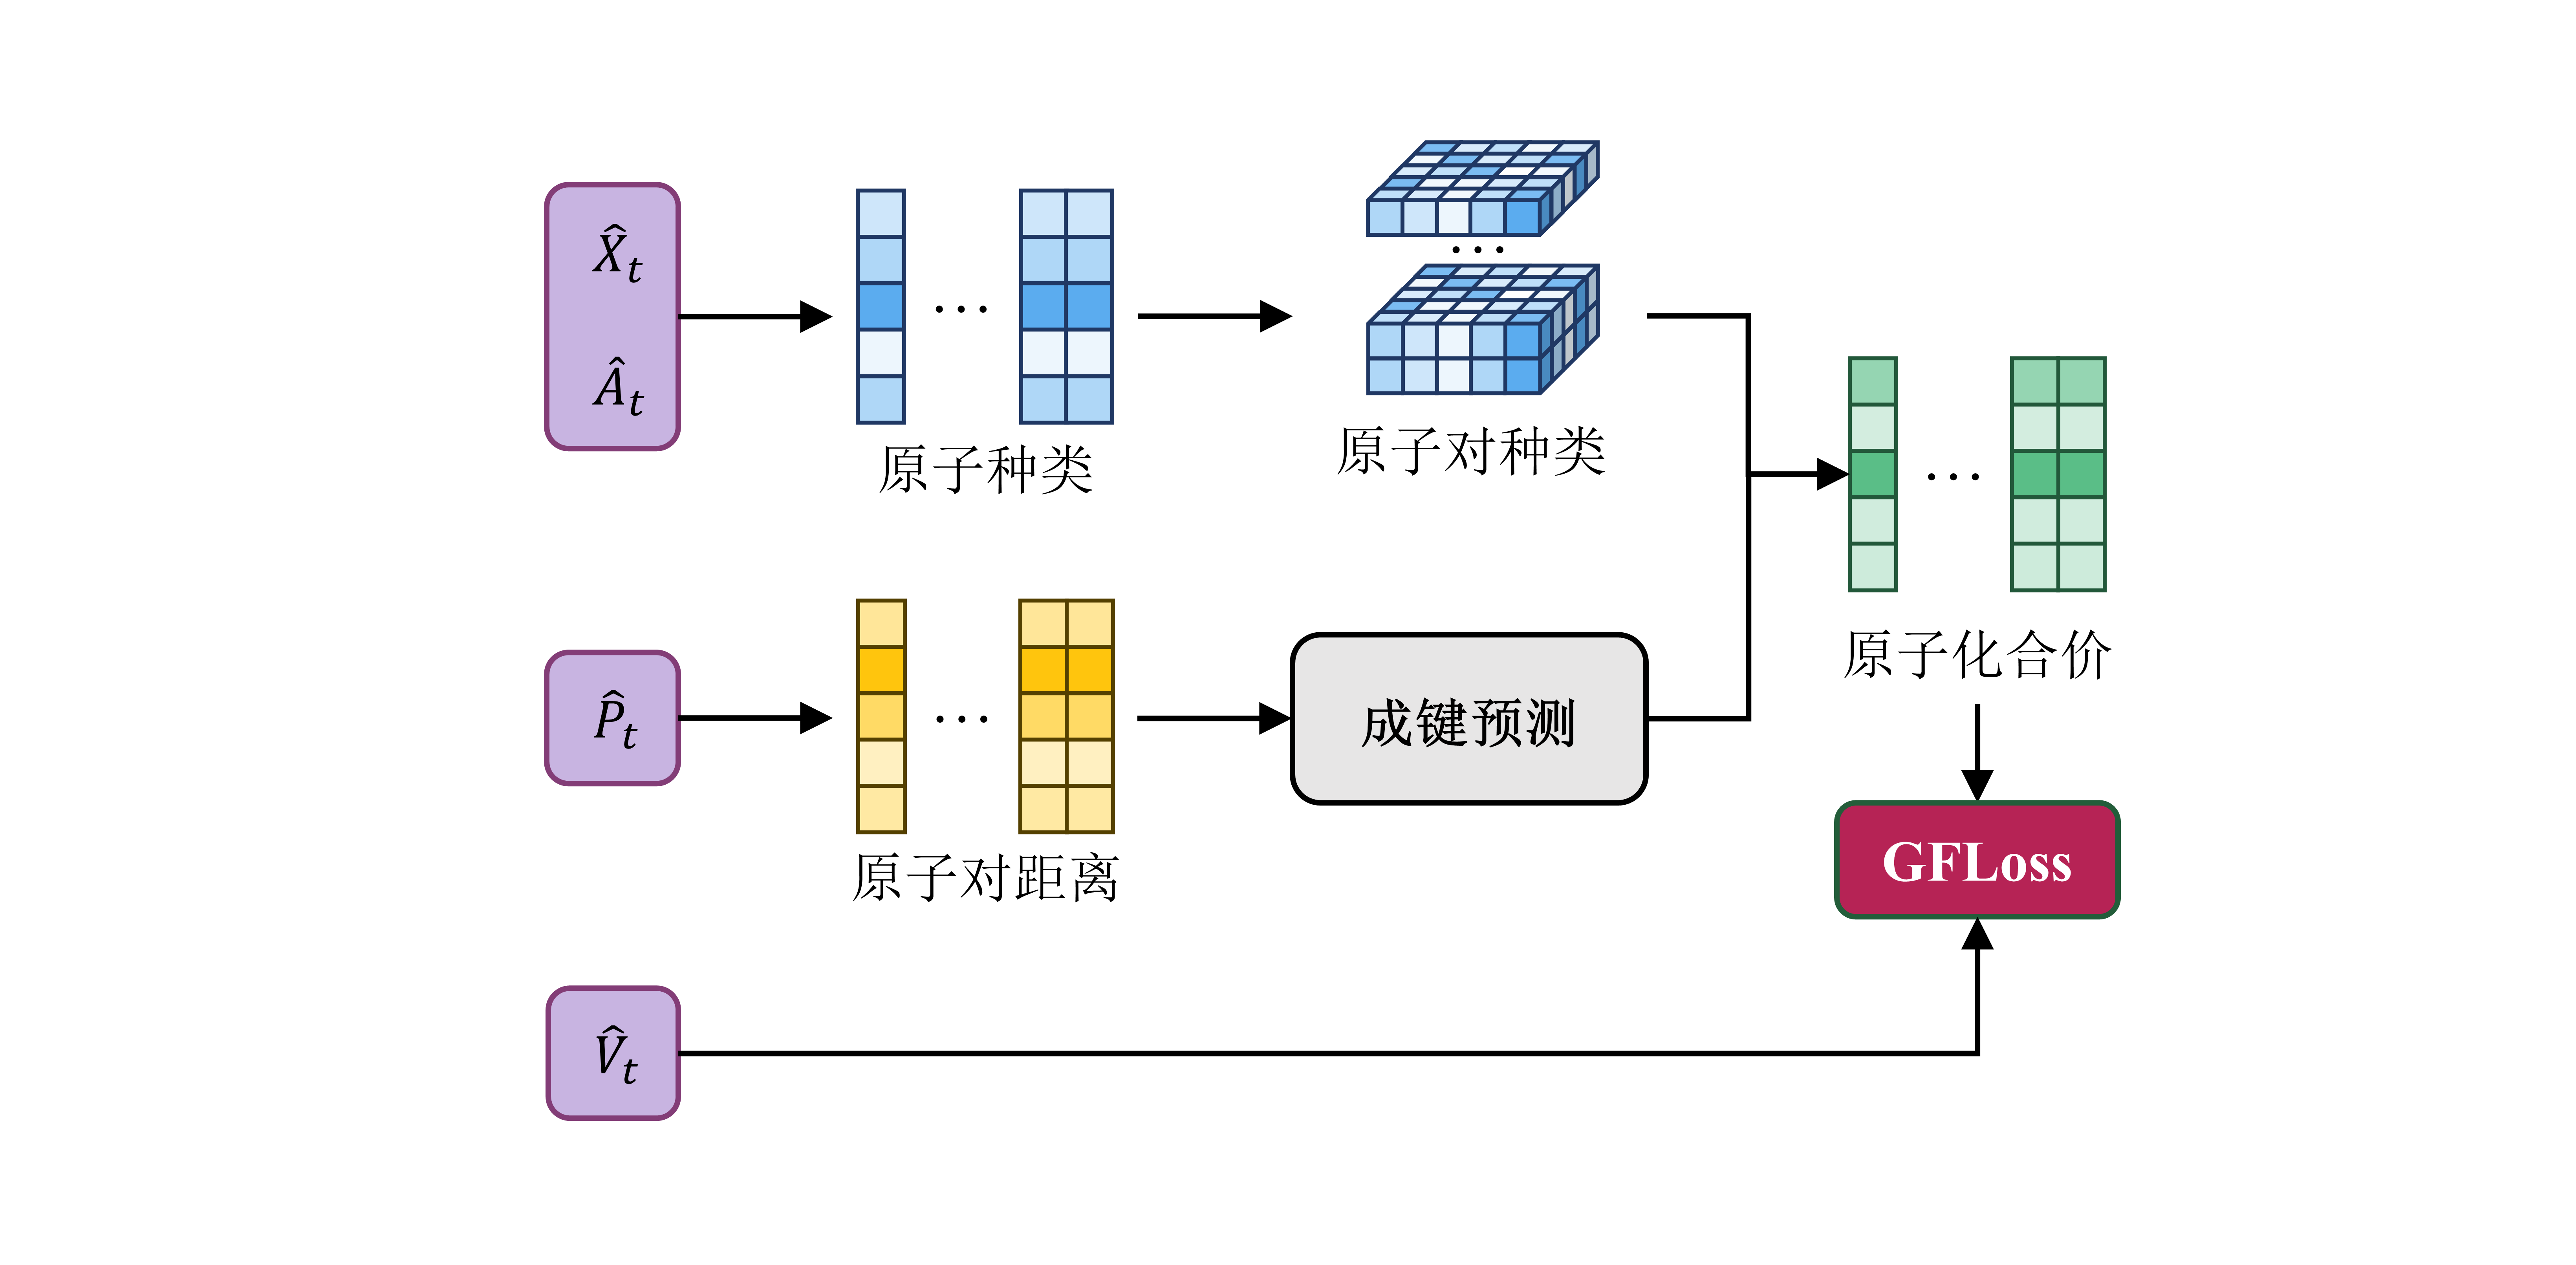
\includegraphics[width=\linewidth]{figures/gfloss.png}
    \caption{GFLoss损失函数}
    \label{fig:gfloss}
\end{figure} 

根据预定义的规则,具有适当距离的原子对间被认为有化学键的存在。对于单键、双键或三键,特定种类的原子之间存在典型距离。如果一对原子之间的距离在某个范围内,这两个原子被认为是由对应类型的键连接的。假设预定义的距离和边界为 $\mathbf{D} \in \mathbb{R}^{nf \times nf \times 3}$ 和 $\mathbf{M} \in \mathbb{R}^{3}$,其中3表示键的类型数量。基于 DTN 的输出 $\hat{G}_t = (\hat{P}_t, \hat{X}_t, \hat{A}_t, \hat{V}_t)$,我们首先使用softmax函数预测原子类型的概率:
\begin{equation}
    {\mathbf{p}}_t(\hat{X}_{{\rm atom}}) = {\rm softmax}(\hat{X}_t) \in \mathbb{R}^{N \times nf},
\end{equation}
其中 $\hat{X}_t$ 在此处表示维度为 $nf$ 的独热编码格式的预测原子类型。原子对的原子类型概率为:
\begin{equation}
    {\mathbf{p}}_t(\hat{X}_{{\rm pair}}) = {\mathbf{p}}_t(\hat{X}_{{\rm atom}}) \cdot {\mathbf{p}}_t(\hat{X}_{{\rm atom}}) \in \mathbb{R}^{N \times N \times nf \times nf}.
\end{equation}

利用DTN预测的原子坐标 $\hat{P}_t$,可以得到原子对距离矩阵 $\mathbf{d}_t \in \mathbb{R}^{N \times N}$,为了方便后续计算,在此需要将其扩展到 $\mathbb{R}^{N \times N \times nf \times nf \times 3}$。为了判断键的存在性,原子对间距与典型的键距离之间的差距 $\mathbf{m}_t$ 计算如下:
\begin{equation}
    \mathbf{m}_t = \mathbf{d}_t - (\mathbf{D} + \mathbf{M}) \in \mathbb{R}^{N \times N \times nf \times nf \times 3}.
\end{equation}
以原子 $i$ 和 $j$ 为例,假设它们被认为是碳原子的概率大于零,如果差距$\mathbf{m}_t(i,j,{\rm C},{\rm C},:)$ 中的任一元素小于零,则表示原子 $i$ 和 $j$ 之间存在一条化学键。化学键的具体类型由差距 $\mathbf{m}_t(i,j,{\rm C},{\rm C},:)$ 中最小值的索引确定。如果 $\arg\min (\mathbf{m}_t(i,j,{\rm C},{\rm C},:))$ 为 1,则化学键判定为单键。如果 $\arg\min (\mathbf{m}_t(i,j,{\rm C},{\rm C},:))$ 为 3,则化学键判定为三键。表示键存在性的布尔矩阵记为 ${\rm ISBOND}_t \in \mathbb{R}^{N \times N \times nf \times nf}$。

一旦我们获得了原子对的原子类型概率和键的存在性预测,就可以估计几何构象决定的原子可能化合价:
\begin{equation}
     \hat{V}_{{\rm pred}}(t) = {\rm sum}({\mathbf{p}}_t(\hat{X}_{{\rm pair}}) \odot {\rm ISBOND}_t) \in \mathbb{R}^{N}.
\end{equation}
由于输入数据受到不同水平噪声的影响,GFLoss被定义为$t$时刻几何构象决定的化合价 $V_{{\rm pred}}(t)$ 与输入样本的真实化合价 $V_t$ 之间的均方误差:
\begin{equation}
    \mathcal{L}_{GF}(t) = ||\alpha_t(\hat{V}_{{\rm pred}}(t) - V_t)||^2,
\end{equation}
其中 $\alpha_t$ 是扩散过程中噪声数据中真实数据的水平。

\begin{algorithm}[H]
    \caption{GFLoss损失函数项伪代码}
    \label{alg:gfloss}
    \begin{algorithmic}
    \STATE {\bfseries Input} 预测的原子序数$\hat{X}_t$,化合价$\hat{V}_t$和几何坐标$\hat{P}_t$;
    \STATE 根据预测的原子序数$\hat{X}_t$计算任一原子类型${\mathbf{p}}_t(\hat{X}_{{\rm atom}})$;
    \STATE 根据任一原子类型计算任一原子对的原子类型${\mathbf{p}}_t(\hat{X}_{{\rm pair}})$;
    \STATE 计算任一原子对距离$\mathbf{d}_t$;
    \STATE 计算原子对距离与3种化学键的典型键长之间的差距$\mathbf{m}_t$;
    \STATE 根据差距$\mathbf{m}_t$判断原子对是否形成某种化学键,并记为布偶型矩阵${\rm ISBOND}_t$;
    \STATE 根据矩阵${\rm ISBOND}_t$和原子对的原子类型${\mathbf{p}}_t(\hat{X}_{{\rm pair}})$计算由几何构象和化学规则
    
    预测的原子化合价$\hat{V}_{{\rm pred}}(t)$;
    \STATE {\bfseries Return} $\mathcal{L}_{GF}(t) = ||\alpha_t(\hat{V}_{{\rm pred}}(t) - V_t)||^2$.
    \end{algorithmic}
\end{algorithm}

\section{扩散及去噪过程}
在提出的GFMDiff的前向过程中,位置、原子序数和原子价逐渐被预设定的噪声先验分布所扰动。对于任一时间步$t = 0, \ldots, T$,需要定义均值$\alpha_t$及方差序列$\sigma_t$。由于 $\alpha_t = \sqrt{1 - \sigma_t^2}$,故实际工程实践中只需定义 $\alpha_t$ 即可。伴随噪声的逐步加入,样本原有的真实信息占比也逐渐减少,故均值序列的值应该单调递减,从 $\alpha_0 \approx 1$ 开始递减,最终到达 $\alpha_T \approx 0$。在本文中,我们设定
\begin{eqnarray}
    &\alpha_t = (1 - 2s) \cdot f(t) + s, & \\
    &f(t) = (1 - (t/T)^2)& 
\end{eqnarray}

为避免数值不稳定情况,序列的数值精度$s$取 $10^{-5}$。该序列设定与\cite{impddpm_nichol_21}中引入的余弦噪声序列较为相似,但本文使用的序列在形式上更为简洁。为了避免采样过程中的数值不稳定性,我们遵循先前研究的\cite{impddpm_nichol_21}的剪切过程,并得到$\alpha_{t|t-1} = \alpha_t / \alpha_{t-1}$,其中$\alpha_{-1} = 1$。在剪切过程中,$\alpha_{t|t-1}^2$的值被剪切到下限$0.001$。这样做确保了$1 / \alpha_{t|t-1}$现在在采样过程中有界,避免采样过程中数值不稳定性。而后,$\alpha_t$ 的值可以使用累积乘积 $\alpha_t = \prod_{\tau=0}^t \alpha_{\tau|\tau-1}$来重新计算。

在方差序列中,$\mathrm{SNR}(t) = \alpha_t^2 / \sigma_t^2$。参照相关研究\cite{vaediff_kingma_21},本文计算负对数$\mathrm{SNR}$曲线为$\gamma(t) = -(\log \alpha_t^2 - \log \sigma_t^2)$,其作为一个单调递增的函数,对高精度数值计算由重要作用。例如,$\alpha_t^2 = \mathrm{sigmoid}(-\gamma(t))$,$\sigma_t^2 = \mathrm{sigmoid}(\gamma(t))$,以及 $\mathrm{SNR}(t) = \exp(-\gamma(t))$,都可以通过对$\gamma(t)$变形得到。

通过具有预定义方差序列$\beta_t \in (0, 1), t=0, 1, ..., T$的马尔可夫链将真实构象$G_0 = (P_0, X_0, A_0, V_0)$进行转换。后验分布定义为:
\begin{eqnarray}
    &q(G_{1:T}|G_0) = \prod^T_{t=1} q(G_t|G_{t-1}),& \\
    &q(G_t|G_{t-1}) = \mathcal{N}_p(p_t;\sqrt{\alpha_t} p_{t-1}, \beta_t I) \cdot \mathcal{N}_h(h_t;\sqrt{\alpha_t} h_{t-1}, \beta_t I),&
\end{eqnarray}
为方便起见,其中$h_t = {\rm concat}(x_t, a_t, v_t)$表示原子特征。

为了在去噪过程中的满足几何坐标的等变性要求,在将原子坐标引入扩散之前,它们必须先转换到质心为零的线性子空间内\cite{enf_satorras_21,edm_hoogeboom_22,geodiff_xu_22}。因此,噪声分布和上述后验分布都受限于相同的线性子空间。此外,原子特征对于对神经网络是等变的,故它们不需要进一步处理即可在整个前向和后向过程中与几何坐标一起进行运算。

考虑欧几里得变量$\mathbf{p} \in \mathbb{R}^{M \times n}$在线性子空间上满足$\sum_i \mathbf{x}_i = \mathbf{0}$。故可以认为$\mathbf{p}$是$n$维空间内的一个质心为零的点云。对于在此子空间上的一个正态分布$\mathcal{N}_x$,欧式变量服从的分布可以表示为:
\begin{equation}
    \mathcal{N}_x(\mathbf{x} | \mathbf{\mu}, \sigma^2 I) = (\sqrt{2 \pi} \sigma)^{-(M-1)\cdot n} \exp \left( -\frac{1}{2\sigma^2} || \mathbf{x} - \mathbf{\mu}||^2 \right),
\end{equation}
其中$\mathbf{\mu}$位于与$\mathbf{x}$相同的子空间中。从这个正态分布中采样有多种方法,例如可以从维度为$(M-1)\cdot n$的正态分布中采样,然后将采样映射到$M\cdot n$维的环境空间中,使得它的重心为零。但是还有一种更简单的方法:可以直接在$M\cdot n$维的环境空间中进行采样,并减去$\sum_i \mathbf{x}_i$。由于正态分布是各向同性的(即无论选择哪个方向,其方差都是 $\sigma^2$),故本文采用这样的方法对原子几何坐标进行采样。

在去噪过程中,我们使用上述的去噪核函数来逼近每个时间步的分子构象,
\begin{eqnarray}
    &p_\theta(G_{t-1}|G_t) = \mathcal{N}(G_{t-1}; \mu_\theta(G_t,t),\sigma_t^2 I),& \\
    &\hat{G}_t = G_t / \alpha_t - \hat{\epsilon}_t \times \sigma_t / \alpha_t ,&
\end{eqnarray}
其中$\hat{\epsilon}_t$是参数化神经网络的输出。

\section{目标函数与评价指标}

对于DDPMs,典型的目标函数是数据对数似然的变分下界。在先前相关研究方法的基础上,我们将目标函数与GFLoss相结合:
\begin{equation}
    \mathcal{L}_t = E_{\epsilon_t \sim \mathcal{N}(0, I)} \left[ \frac{1}{2} \omega(t) \left( ||\epsilon_t - \hat{\epsilon}_t||^2 + \lambda || \alpha_t(\hat{V}_{pred}(t) - V_t)||^2 \right) \right],
\end{equation}
其中$\omega(t) = (1-{\rm SNR}(t)/{\rm SNR}(t-1))$。

此外,在评价模型参数的好坏时,需要比较模型学习的去噪分布于前向噪声分布的差异。该指标具体表现为参数的负对数似然函数,由于负对数似然函数无法直接计算得到,本文通过算法~\ref{alg:nll_gfmdiff}~估计该负对数似然函数的取值。

\begin{algorithm}[H]
    \caption{GFMDiff参数的负对数似然函数估计}
    \label{alg:nll_gfmdiff}
    \begin{algorithmic}
    \STATE {\bfseries Input} 原子坐标$p$,原子特征$h = [x, a, v]$,去噪神经网络$\phi$;
    \STATE 采样时间步 $t \sim \mathcal{U}(1, T)$和噪声 $\varepsilon_t = [\varepsilon^{(p)}_t, ~\varepsilon^{(h)}_t] \sim \mathcal{N}(\mathbf{0}, I)$;
    \STATE 混合输入样本与噪声 $z_t = \alpha_t [p, h] + \sigma_t \varepsilon_t$;
    \STATE 计算神经网络损失函数 $\mathcal{L}_t = \frac{1}{2}(1 - \mathrm{SNR}(t-1) / \mathrm{SNR}(t)) ||\varepsilon_t - \phi(z_t, t)||^2$;
    \STATE 采样0时刻样本噪声 $\varepsilon_0 = [\varepsilon^{(p)}_0, ~\varepsilon^{(h)}_0] \sim \mathcal{N}(\mathbf{0}, I)$;
    \STATE 混合0时刻输入样本与噪声 $z_0 = \alpha_0 [p, h] + \sigma_0 \varepsilon_0$;
    \STATE 计算0时刻损失函数 $\mathcal{L}_0 = \mathcal{L}_0^{(x)} + \mathcal{L}_0^{(h)} = -\frac{1}{2} ||\varepsilon_0 - \phi(z_0, 0)||^2 - \log Z + \log p(h | z_0^{(h)})$;
    \STATE $\mathcal{L}_{\text{base}} = -\mathrm{KL}(q(z_T | x, h) | p(z_T)) = -\mathrm{KL}(\mathcal{N}_{xh}(\alpha_T [x, h], \sigma_T^2 I) | \mathcal{N}_{xh}(\mathbf{0}, I))$;
    \STATE {\bfseries Return} $\hat{\mathcal{L}} = T \cdot \mathcal{L}_t + \mathcal{L}_0 + \mathcal{L}_{\text{base}}$.
    \end{algorithmic}
\end{algorithm}

其中对于前向和反向过程的样本KL散度的计算,无法直接得到。对于两个各向同性正态分布$q = \mathcal{N}(\mathbf{\mu}_1, \sigma_1^2 I)$和$p = \mathcal{N}(\mathbf{\mu}_2, \sigma_2^2 I)$,标准的KL散度可表示为:
\begin{equation}
    \mathrm{KL}(q || p) = d \cdot \log \frac{\sigma_2}{\sigma_1} + \frac{1}{2} \left[ \frac{d \cdot \sigma_1^2 + ||\mathbf{\mu}_1 - \mathbf{\mu}_2||^2}{\sigma_2^2} - d  \right],
\end{equation}
其中$d$是分布的维度。在扩散模型中,扩散过程和去噪过程具有相同的方差$\sigma^2$。如果$\sigma_1 = \sigma_2 = \sigma$,则这两个分布的KL散度可简化为:
\begin{equation}
    \mathrm{KL}(q || p) = \frac{1}{2} \left[ \frac{||\mathbf{\mu}_1 - \mathbf{\mu}_2||^2}{\sigma^2} \right].
    \label{eqn:kl1}
\end{equation}

现假设$\mathcal{N}_1(\tilde{\mathbf{\mu}}_1, \sigma^2 I)$和$\mathcal{N}_2(\tilde{\mathbf{\mu}}_2, \sigma^2 I)$在一个线性子空间上,其中均值 $\tilde{\mathbf{\mu}}$ 是相对于子空间中的任意坐标系定义的,则这两个分布之间的KL散度包含一个包含欧几里得距离项$||\tilde{\mathbf{\mu}}_1 - \tilde{\mathbf{\mu}}_2||^2$。

类似于E-NF\cite{enf_satorras_21}和GeoDiff\cite{geodiff_xu_22}中的论证,可以构造一个正交变换$Q$,将满足$\sum_i \mathbf{\mu}_i = \mathbf{0}$条件的环境空间映射到子空间上,以满足$\begin{bmatrix} \tilde{\mathbf{\mu}} \\ \mathbf{0} \end{bmatrix} = Q \mathbf{\mu}$。由于$||\tilde{\mathbf{\mu}}|| = ||\begin{bmatrix} \tilde{\mathbf{\mu}} \\ \mathbf{0} \end{bmatrix}|| = ||\mathbf{\mu}||$,故$||\tilde{\mathbf{\mu}}_1 - \tilde{\mathbf{\mu}}_2||^2 = ||\mathbf{\mu}_1 - \mathbf{\mu}_2||^2$。这表明式~\ref{eqn:kl1}~在环境空间内可以通过计算得到。
% 这同样表明在某些扩散模型中,后验扩散过程和去噪过程使用的方差不同。从方程可以看出,KL散度取决于子空间的维度,而不是环境空间的维度。

对于诸如$\mathcal{N}$这样的分布,只要两个分布之间的方差相同,KL散度仍然可以在环境空间中计算。现在考虑分布$q = \mathcal{N}_{ph}(\mathbf{\mu}_1, \sigma^2 I)$和$p = \mathcal{N}_{ph}(\mathbf{\mu}_2, \sigma^2 I)$ 的组合KL散度。注意到这里的均值由两部分组成 $\mathbf{\mu} = [\mathbf{\mu}^{(p)}, \mathbf{\mu}^{(h)}]$,其中$p$部分位于一个子空间中,而$h$作为原子特征分布没有特定要求。因此该分布可以分解为$\mathcal{N}_{ph}(\mathbf{\mu}, \sigma^2 I) = \mathcal{N}_{p}(\mathbf{\mu}^{(p)}, \sigma^2 I) \cdot \mathcal{N}(\mathbf{\mu}^{(h)}, \sigma^2 I)$。因此扩散和去噪过程样本分布的KL散度可以被简化为:
\begin{align}
    \begin{split}
        \mathrm{KL}(q||p) &= \mathrm{KL}\left(\mathcal{N}_{p}(\mathbf{\mu}_1^{(p)}, \sigma^2 I) || \mathcal{N}_{p}(\mathbf{\mu}_2^{(p)}, \sigma^2 I)\right) + \mathrm{KL}\left(\mathcal{N}(\mathbf{\mu}_1^{(h)}, \sigma^2 I) || \mathcal{N}(\mathbf{\mu}_2^{(h)}, \sigma^2 I )\right) \\
        &= \frac{1}{2} \left[ \frac{||\mathbf{\mu}_1^{(p)} - \mathbf{\mu}_2^{(p)}||^2}{\sigma^2} \right] + \frac{1}{2} \left[ \frac{||\mathbf{\mu}_1^{(h)} - \mathbf{\mu}_2^{(h)}||^2}{\sigma^2} \right] = \frac{1}{2} \left[ \frac{||\mathbf{\mu}_1 - \mathbf{\mu}_2||^2}{\sigma^2} \right].
    \end{split}
\end{align}


    \chapter{实验结果及分析}
\label{chap:experiment}

在此部分,本文将首先全方位检验提出的用于创新3D药物分子设计的几何促进的分子扩散框架GFMDiff在生成3D分子任务中的表现,用于性能比较的三个任务和两个公开数据集都具备极强的代表性。同时为了进一步探究本文提出的DTN去噪内核作为分子学习模型,在分子性质预测任务上的表现。本文将DTN与时下性能最优的3D分子学习模型,在2个公开数据集上的表现进行对比。

\section{药物分子设计}
在本节中,我们报告了GFMDiff在两个主流数据集GEOM-QM9 \cite{qm9_ramakrishnan_14}和GEOM-Drugs \cite{drugs_axelrod_22}上的三个生成任务中的表现。本文采用了时下最前沿的相关研究模型作为基线模型,在采取一致的实验条件的前提下,直接引用他们生成的实验结果。结果表明,我们的方法在多个方面显著优于该领域最优秀的模型,展现出在3D分子生成任务中时下最优的性能。

\subsection{实验设置}

\textbf{数据集:}
为了进行全面且公平的比较,我们在两个基准数据集(GEOM-QM9和GEOM-Drugs)上进行了三组实验:在GEOM-QM9上的药物分子设计,在GEOM-QM9上有条件的药物分子设计,和在GEOM-Drugs上的药物分子设计。具体的数据集处理工作较为琐碎,本文将在对应的生成任务实验分析中分别介绍。

GEOM-QM9数据集(简称:QM9)是一个广泛运用在基于深度学习的分子学习领域的数据集,包含超过13万个分子及其对应的构象,以及每个分子对应的19种性质。数据集中,在包含氢原子条件下,平均每个分子有19个原子,其中最大的分子有29个原子。同时,整个数据集的分子仅包括氢,碳,氮,氧,氟这五种原子。

GEOM-Drugs(简称:Drugs)是一个规模相对更大的数据集,其包括的分子数量和每个分子所含平均原子数都较多。该数据集记录了超过45万个分子和它们对应的3700万个不同构象。在包含氢原子的条件下,平均每个分子由44个原子构成,最大的由181个原子构成。同时,整个数据集的分子包含16类原子,较QM9比原子种类更丰富。

\textbf{评价指标:}
为公平的评价GFMDiff的性能并与时下最优秀的模型对比,本文采用目前该领域通用的评价指标,具体介绍如下。

$\bullet$ 负对数似然函数(Negative log-likelihood / NLL):是一个被广泛应用于评价参数估计的指标,其在深度学习中也可以被用作损失函数。

$\bullet$ 稳定性(Stability):是3D分子设计领域最重要的评价指标,其衡量了生成的分子构型和化学键在几何空间内是否稳定。对于一个化学键而言,根据其两端连接的原子的类型和化学键类型的不同,在计算化学上存在不同的理想稳定键长\footnote{\url{http://www.wiredchemist.com/chemistry/data/bond_energies_lengths.html}}\footnote{\url{https://www.mrbigler.com/documents/Chemistry_Reference_Tables.pdf}}。例如对两个碳原子,其可能形成单键,双键和三键。对于碳碳单键,双键和三键,其理论键能分别为346,602,835(千焦/摩尔),对应键长分别为154,134,120(皮米)。对于模型生成的分子几何构象,若一对碳原子间距离小于120皮米,则认为这两个碳原子由三键连接,若距离大于120皮米,且小于134皮米,则认为它们由双键连接。若原子间距离超过154皮米,则认为两者之间不存在键相连。根据计算化学相关知识,若一个原子经过预测,连接的所有键总计化合价预期理论值一致,则认为该原子稳定。以碳原子为例,若其经过预测后与4个其他原子形成单键,或形成2个单键1个双键,则认为该碳原子是稳定的。如果一个分子中所有的原子都具备正确的化合价,则该分子也被认为是稳定的。该指标有效的同时衡量生成的三维分子构象的几何和拓扑性质。在具体评价中,稳定性可分为原子稳定性(Atom Stability)和分子稳定性(Molecule Stability),他们各自代表稳定原子/分子在所有原子/分子中的数量占比。

$\bullet$ 有效性(Validity):是在2D和3D分子生成领域通用的评价指标,其衡量了有效分子在所有分子中的数量占比。 一个分子的有效与否,决定于RDKit中对分子中化合价和度的判断。

$\bullet$ 唯一性(Uniqueness):同样对2D和3D分子设计通用,该指标衡量了生成结果中非重复的分子的数量占比。

$\bullet$ 平均绝对误差(Mean absolute error / MAE):是一个常用于回归任务的评价指标。在本文中,该指标仅用于评价有条件的分子生成的样本属性。

\textbf{基线模型:}
本文采用了本领域最具代表性且最前沿的模型,包含基于自回归模型的,流型模型的和扩散模型的方法。

$\bullet$ E-NF\cite{enf_satorras_21}是基于流型模型的3D分子设计的模型。其中用于图学习的网络为等变的EGNNs\cite{egnn_satorras_21}。该网络将原子间距离视作键的特征,通过信息传递更新相应节点特征。

$\bullet$ G-SchNet\cite{gschnet_wallach_19}在SchNet\cite{schnet_schutt_17}的基础上设计了一个自回归模型,通过逐步生成原子和键的方式生成分子结构。SchNet已经被证明其对角度信息具备良好提取能力。

$\bullet$ EDM\cite{edm_hoogeboom_22}是最早将扩散模型引入到药物分子设计的模型。其去噪内核同样采用EGNNs\cite{egnn_satorras_21}。

$\bullet$ Bridge和Bridge+Force\cite{diffpg_wu_22}提出能量方式用于更有效的引入几何信息,通过分子间作用力,引导分子生成更有效更稳定的构型。

$\bullet$ GCDM\cite{gcdm_morehead_23}是距今该领域表现最好且拥有完整开源代码的方法。其参照ColfNet的思路\cite{colfnet_du_22}引入了完整的空间几何信息。

为了公平客观的评价GFMDiff的性能,本文选取的基线模型都是具备完整可复现开源代码的模型,并在采用一致基本参数设置的条件进行实验。本文引用了EDM\footnote{\url{https://github.com/ehoogeboom/e3_diffusion_for_molecules}}实验部分中E-NF,G-SchNet和EDM的表现,引用了Bridge和Bridge+Force的实验结果,以及GCDM\footnote{\url{https://github.com/BioinfoMachineLearning/bio-diffusion}}的实验结果。

\textbf{实验环境:}
本文在生成实验上基于的硬件平台如下:

GEOM-QM9实验:Intel(R) Xeon(R) Platinum 8358和2 * NVIDIA A100 SXM4 40GB; 

GEOM-Drugs实验: AMD EPYC 7742和4 * NVIDIA A100 PCIe 80GB。

此外,相关实验依赖的一些重要的包有:CUDA 11.4,Python 3.9.13,PyTorch 1.10.0,PyG 2.0.4,RDKit 2022.03.5。

\subsection{在GEOM-QM9上的药物分子设计}
\begin{table}[h]
    \centering
    \caption{GEOM-QM9上药物分子设计结果对比}
    \label{tab:gen_qm9}
    \begin{tabular}{lllllll}
    \toprule
    Type & Method & NLL$\downarrow$ & \makecell[l]{Atom\\Stability\\(\%) $\uparrow$} & \makecell[l]{Mol\\Stability\\(\%) $\uparrow$} & \makecell[l]{Validity\\(\%) $\uparrow$} & \makecell[c]{Uniqueness\\$\times$\\Validity(\%) $\uparrow$} \\
    \midrule
    NF & E-NF & -59.7 & 85.0 & 4.9 & 40.2 & 39.4 \\
    \cline{2-7}
    AR & G-SchNet & N/A & 95.7 & 68.1 & 85.5 & 80.3 \\
    \cline{2-7}
    \multirow{2}{*}{DDPM}
    & EDM & -110.7$\pm$1.5 & 98.7$\pm$0.1 & 82.0$\pm$0.4 & 91.9$\pm$0.5 & 90.7$\pm$0.6 \\
    & Bridge & N/A & 98.7$\pm$0.1 & 81.8$\pm$0.2 & N/A & N/A \\
    & Bridge+Force & N/A & \underline{98.8}$\pm$0.1 & 84.6$\pm$0.3 & N/A & N/A \\
    & GCDM & \textbf{-171.0}$\pm$0.2 & 98.7$\pm$0.0 & 85.7$\pm$0.4 & 94.8$\pm$0.2 & 93.3$\pm$0.0 \\
    \midrule
    \multirow{2}{*}{\makecell[l]{DDPM\\(Ours)}} & \makecell[l]{GFMDiff\\w/o tri} & -123.1$\pm$0.4 & 98.7$\pm$0.1 & 85.9$\pm$0.2 & 94.9$\pm$0.2 & 94.2$\pm$0.2 \\
    & \makecell[l]{GFMDiff\\w/o GFLoss} & -127.5$\pm$0.4 & 98.7$\pm$0.0 & \underline{87.5}$\pm$0.1 & \underline{96.0}$\pm$0.0 & \underline{95.2}$\pm$0.0 \\
    & GFMDiff & \underline{-132.5}$\pm$0.2 & \textbf{99.1}$\pm$0.0 & \textbf{91.3}$\pm$0.2 & \textbf{97.0}$\pm$0.3 & \textbf{96.1}$\pm$0.2 \\
    \midrule
    Data &  &  & 99.0 & 95.2 & 97.7 & 97.7 \\
    \bottomrule
    \end{tabular}
\end{table}
\begin{figure}[h]
    \centering
    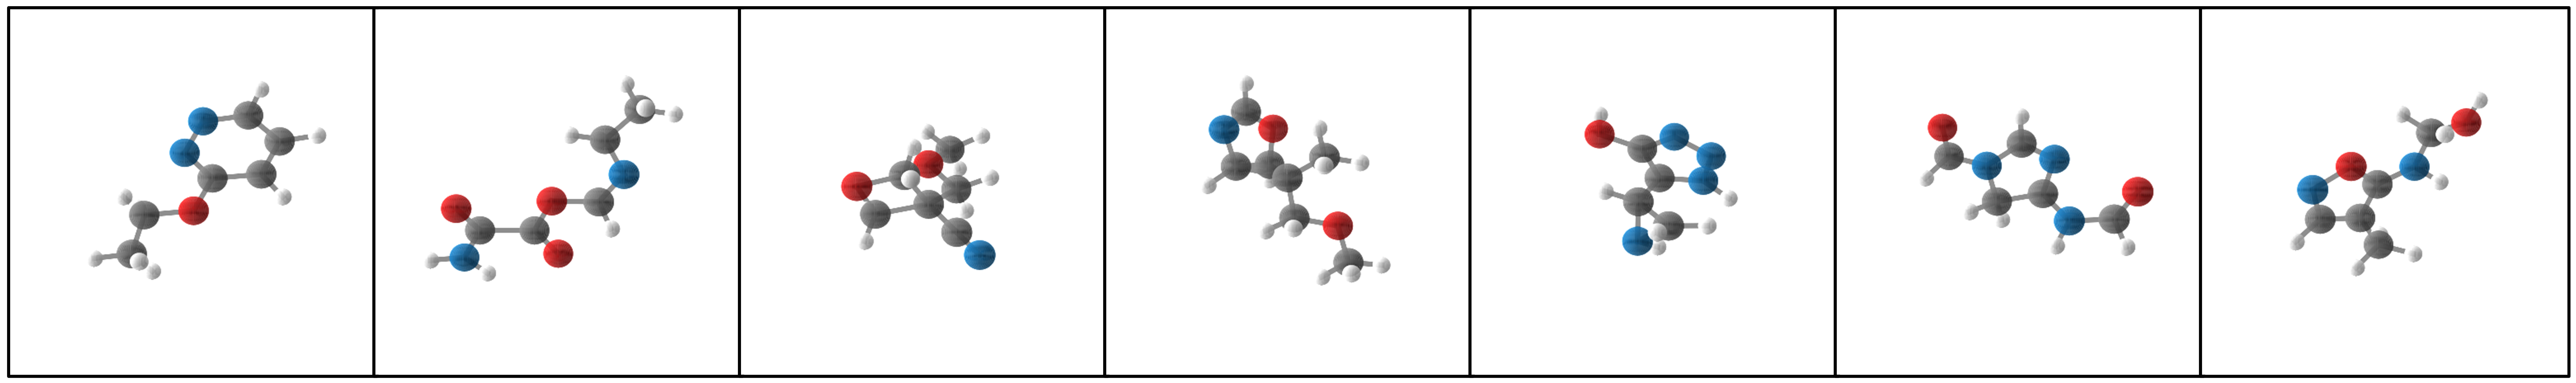
\includegraphics[width=\linewidth]{figures/samples_qm9.png}
    \caption{GFMDiff在GEOM-QM9上药物分子设计样本示意}
    \label{fig:samples_qm9}
\end{figure}

在该任务的实验中,本文依照先前研究,将QM9数据集分别划分为样本大小为10万,1.8万和1.3万的训练集,验证集和测试集。表~\ref{tab:gen_qm9}~为GFMDiff和基线模型在分子在QM9数据集上的表现对比,指标旁的箭头代表更优取值的方向。同时图~\ref{fig:samples_qm9}~展示了部分生成分子的三维构象。NLL的取值为模型在测试集上的得分,而剩余指标的计算基于模型随机生成的10000个样本。此外,部分基线模型的特定指标可能在先前研究没有说明,在此用N/A替代。在表中,最好和次好的结果分别以粗体和下划线的形式予以强调。

除了在测试集上的NLL得分,本文在其他的所有指标上都显著优于基线模型。稳定性作为创新3D药物分子设计任务中的核心指标,GFMDiff在这两个评价指标中较先前研究有明显优势,分子稳定性较表现最好的基线模型有6.5\%的提升,这证明了GFMDiff对几何信息的有效利用极大的提升了模型性能。在有效性层面,GFMDiff较表现最好的基线模型的提升分别为2.3\%和3\%。这说明了GFMDiff能够生成有效且非重复的分子。值得一提的是,GFMDiff生成结果已经十分接近,甚至在个别指标上超过了数据本身,实验结果充分表明了本文提出的GFMDiff在生成中型分子时具备的优异性能。

为衡量本文提出的的DTN去噪内核和GFLoss损失函数的有效性,本文进行了两组消融实验。在此,将GFLoss损失函数的权重$\lambda$设置为0,则可以得到GFMDiff w/o GFLoss模型。在此基础上,本文将DTN中原子对-三元组间的注意力机制模块取代为一个原子对自注意力机制模块,得到GFMDiff w/o tri模型。GFMDiff w/o GFLoss消融实验的结果表明本文引入的GFLoss损失函数对生成稳定、有效的药物分子三维构象有积极促进作用。其在评价指标上全面落后于GFMDiff。GFMDiff w/o tri模型的结果较另外两个GFMDiff模型有更大的降幅。这样的结果表明DTN中对分子三元组信息的提取,并将其融入原子对距离学习是有效的。作为表现最差的GFMDiff模型变体,该模型仍优于其他基线模型,这也足以说明双轨Transformer网络中的双轨设计和基于Transformer的分子图学习的有效性。

\subsection{在GEOM-QM9上有条件的药物分子设计}
除了最基本的稳定性和有效性,生成具备良好属性的药物分子是药物分子生成模型应当具备的一项能力。为评价模型在有条件的药物分子生成任务上的表现,本文根据通行做法开展实验。在QM9数据集包含的所有性质中,选取各向同性极化率$\alpha$,最高占据分子轨道$\varepsilon_{{\rm HOMO}}$,最低未占分子轨道$\varepsilon_{{\rm LUMO}}$,两者间能量隙$\Delta \varepsilon$,偶极矩$\mu$和298.15K时的热容$C_v$。

\begin{table}[h]
    \centering
    \caption{GEOM-QM9上有条件的药物分子设计结果对比}
    \label{tab:gen_qm9_condition}
    \begin{tabular}{lllllll}
    \toprule
    \makecell[l]{Task\\Units} & \makecell[l]{$\alpha$\\${\rm Bohr^3}$} & \makecell[l]{$\Delta \varepsilon$\\${\rm meV}$} & \makecell[l]{$\varepsilon_{{\rm HOMO}}$\\${\rm meV}$} & \makecell[l]{$\varepsilon_{{\rm LUMO}}$\\${\rm meV}$} & \makecell[l]{$\mu$\\${\rm D}$} & \makecell[l]{$C_v$\\$\frac{{\rm cal}}{{\rm mol}}{\rm K}$} \\
    \midrule
    Naive (Upper-bound) & 9.01 & 1470 & 645 & 1457 & 1.616 & 6.857 \\
    \# Atom & 3.86 & 866 & 426 & 813 & 1.053 & 1.971 \\
    EDM & 2.76 & 655 & 356 & 584 & 1.111 & 1.101 \\
    GCDM & \underline{1.97} & \underline{602} & \underline{344} & \underline{479} & \underline{0.844} & \underline{0.689} \\
    GFMDiff & \textbf{1.74} & \textbf{558} & \textbf{321} & \textbf{430} & \textbf{0.728} & \textbf{0.593} \\
    QM9 (Lower-bound) & 0.10 & 64 & 39 & 36 & 0.043 & 0.040 \\
    \bottomrule
    \end{tabular}
\end{table}

\begin{figure}[h]
    \centering
    \includegraphics[width=\linewidth]{figures/samples_qm9_cond.png}
    \caption{GFMDiff在GEOM-QM9上有条件的药物分子设计样本示意}
    \label{fig:samples_qm9_cond}
\end{figure}

为检验生成的药物分子是否具备良好属性,在实验时,需要将QM9数据集的训练集部分平均分为两部分。在训练阶段,第一部分被用作一个EGNN\cite{egnn_satorras_21}神经网络的训练。该网络通过学习正确的分子及对应的属性,故将具备根据输入分子预测相应性质的能力。第二部分数据集被用作生成模型的训练,即在普通的生成模型基础上,在训练时增加对应性质信息。在两部分都完成训练后,则预先根据训练集中性质的均值和方差,采样得到需要生成样本具备的性质。根据这部分性质,生成模型会生成10000个采样结果。这部分采样结果将通过之前训练好的EGNN神经网络,进行对应的性质预测,最终的衡量标准为EGNN预测的分子性质和分子生成时依照的性质间的平均绝对误差。

在基线模型上,本文引入了三个参照模型:Naive,\#Atom和QM9。Naive模型在测试阶段时,EGNN模型根据随机打乱原有的采样样本对应性质并预测相应结果,这代表了在此任务下预测结果MAE的取值上限。\#Atom模型在测试阶段,EGNN模型仅依据分子所含原子数对性质进行预测。如果生成模型的测试MAE较\#Atom模型低,则说明该模型能够根据特定性质生成相应的分子。参照模型QM9则代表EGNN在QM9数据集上的预测性能,该表现代表分子性质预测结果的MAE下界。

根据表~\ref{tab:gen_qm9_condition}~所示,本文提出的GFMDiff在测试任务中预测结果的MAE均低于目前最优的GCDM模型,在所有六个指标中的领先幅度分别为:11.7\%,7.3\%,6.7\%,10.2\%和13.7\%。该表现足以证明,GFMDiff具备根据指定条件生成分子的能力。图~\ref{fig:samples_qm9_cond}~中全面的展示了GFMDiff依据不同的性质取值,生成对应的药物分子样本。以各向同性极化率$\alpha$为例,随着$\alpha$取值增加,模型倾向于生成更长的碳链。

\subsection{在GEOM-Drugs上的药物分子设计}
在GEOM-Drugs数据集基础上进行创新药物分子设计是一个具有挑战性的任务,因为该数据集不仅包含分子多,也因其中分子主要为大分子,这对分子图中键的形成提出了较高的要求。在对GEOM-Drugs的实验中,我们将GFMDiff与E-NF、EDM、Bridge+Force和GCDM进行了比较。此外,由于当前方法面对如此庞大且自身数据不够精良的生成任务时,较QM9数据集上的表现有较大差距,常常无法生成新的分子,故在此讨论生成分子的有效性是缺乏意义的。在评价指标方面,本文采用了生成10000个药物分子的稳定性用作性能比较。

\begin{table}[h]
    \centering
    \caption{GEOM-Drugs上药物分子设计结果对比}
    \label{tab:gen_drugs}
    \begin{tabular}{llll}
    \toprule
    Type & Method & Atom Stability (\%) $\uparrow$ & Mol Stability (\%) $\uparrow$ \\
    \midrule
    Normalizing flow & E-NF & 75.0 & 0 \\
    \multirow{2}{*}{DDPM}
    & EDM  & 81.3 & 0.0 \\
    & Bridge & 81.0$\pm$0.7 & 0.0 \\
    & Bridge+Force & 82.4$\pm$0.8 & 0.0 \\
    & GCDM & 86.4$\pm$0.2 & 3.7$\pm$0.3 \\
    \midrule
    Ours & GFMDiff & \textbf{86.5}$\pm$0.2 & \textbf{3.9}$\pm$0.2 \\
    \midrule
    Data &  & 86.5 & 2.8 \\
    \bottomrule
    \end{tabular}
\end{table}
\begin{figure}[h]
    \centering
    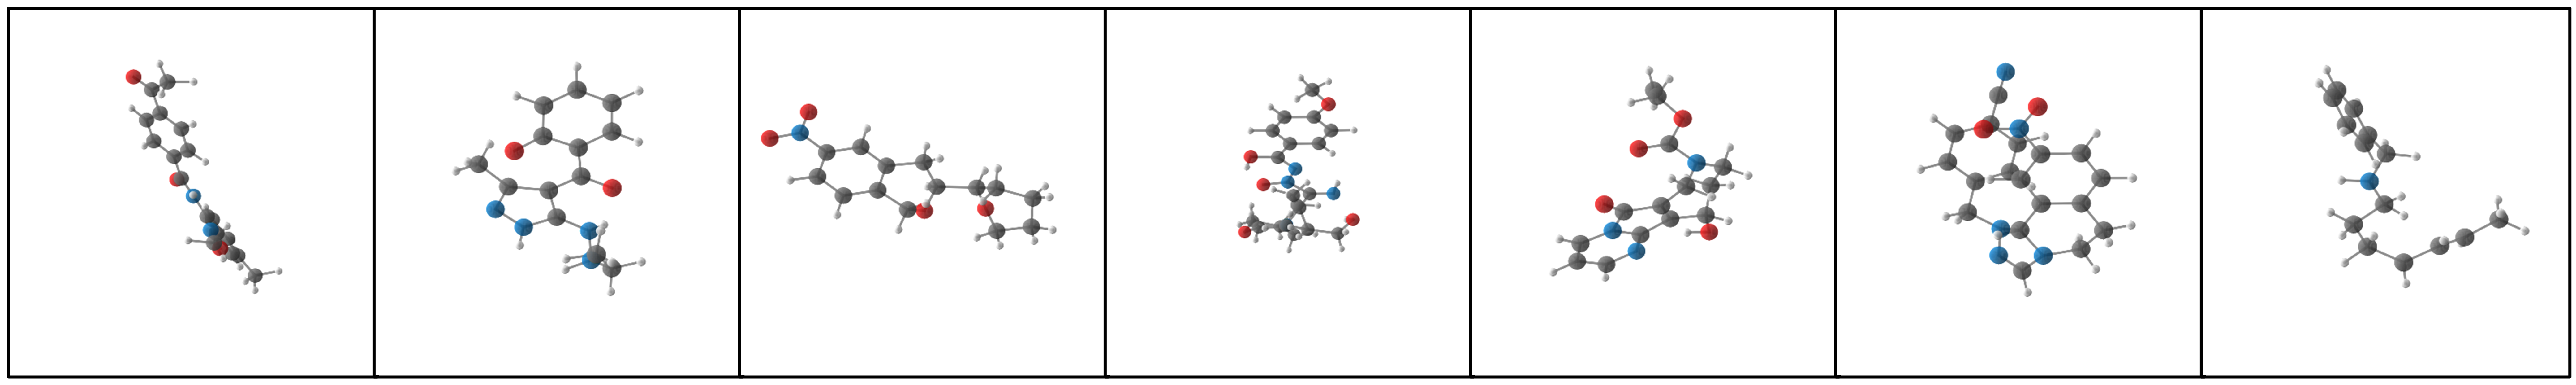
\includegraphics[width=\linewidth]{figures/samples_drugs.png}
    \caption{GFMDiff在GEOM-Drugs上药物分子设计样本示意}
    \label{fig:samples_drugs}
\end{figure}

由于GEOM-Drugs中分子庞大,且该数据集不如QM9精确,其自身的稳定性就比QM9中要低得多。由表~\ref{tab:gen_drugs}~与QM9上实验展现出的优秀表现一致,本文提出的GFMDiff在原子稳定性方面略优于GCDM,同时显著优于其他基线模型。在分子的整体稳定性方面,GFMDiff的表现超过第二名结果5.4\%。图~\ref{fig:samples_drugs}~展示了部分生成分子的三维构象。在Drugs上的结果也足以证明了本文提出的GFMDiff在捕捉三维原子相互作用并生成的分子键时的强大能力。


\section{分子性质预测}
在AI辅助药物发现领域,分子性质预测也是十分基础的研究问题。为验证本文提出的双轨Transformer网络(DTN)对三维分子几何信息的学习能力,本文在两个大型公开分子数据集上进行了全面的实验。

\subsection{实验设置}
\textbf{数据集:}在分子性质预测实验中,本文使用了两个广泛使用的基准公开数据集:OC20和GEOM-QM9。在此,本节只介绍OC20数据集的详细信息。

$\bullet$ Open Catalyst 2020 (OC20) \cite{oc20_chanussot_21}数据集是一个较新的公开大规模数据集,用于建模和发现催化剂。具体而言,其目标是对结构弛豫进行高效的密度泛函理论(Density functional theory / DFT)近似计算。在催化剂研究中,结构弛豫是一项基础计算任务,其被用于确定结构的活性和选择性。数据集中的所有结构都包含一个表面和一个吸附物,表面由一个周期性的晶胞定义。该数据集中包括三个任务,分别是结构到能量和力(S2EF),初始结构到弛豫结构(IS2RS)和初始结构到弛豫能量(IS2RE)。本文中,我们聚焦于初始结构到弛豫能量(IS2RE)任务,这是催化剂研究中最常见的任务,因为弛豫能量通常与催化剂的活性和选择性相关。与相关研究采取的设置类似,本文将IS2RE的数据集分为训练集、验证集和测试集。训练集包含460,328个分子结构,验证集分为域内(ID)、域外吸附物(OOD Ads)、域外催化剂(OOD Cat)和域外吸附物和催化剂(OOD Both)四个子集,分别包含24,733、24,961、24,738、24,971个结构。

\textbf{评价指标:}
在回归任务中,本文主要采取预测结果的MAE作为衡量评价模型预测准确程度的指标。此外在OC20的任务上,本文还引入了真实能量阈值内占比(Energies within a Threshold)作为另一衡量指标。

\textbf{基线模型:}
在基线模型的选择上,本文选取了时下最优的有可复现代码的模型用于性能对比。包括CGCNN \cite{cgcnn_xie_18},SchNet \cite{schnet_schutt_17},PhysNet \cite{physnet_unke_19},MGCN \cite{mgcn_lu_19},DimeNet++ \cite{dimenetpp_gasteiger_20},GemNet \cite{gemnet_gasteiger_21},PaiNN \cite{painn_schutt_21},SphereNet \cite{spherenet_liu_22}和ComENet \cite{comenet_wang_22}。

\subsection{在GEOM-QM9数据集上的分子性质预测}
为检测DTN在分子性质预测上的性能和在量子化学系统中的预测能力,我们将DTN应用于QM9数据集上的分子性质预测任务。表~\ref{tab:reg_qm9}~展示了本文DTN和基线模型在回归任务上结果的MAE对比,任务包括12种性质及所有任务上的总体均方根误差(std. MAE)。其中每项任务表现最佳和次佳的结果分别以粗体和下划线的形式予以强调。

\begin{table}[h]
    \begin{center}
    \caption{GEOM-QM9上药物分子性质预测结果对比}
    \label{tab:reg_qm9}
    \resizebox{\textwidth}{!}
    % \small
    {\begin{tabular}{llcccccccc}
    \toprule
    Property & Unit & SchNet & PhysNet & MGCN & DimeNet++ & PaiNN & SphereNet & ComENet & DTN \\
    \midrule
    $\mu$ & D & 0.033 & 0.0529 & 0.0560 & 0.0297 & \textbf{0.012} & 0.0245 & 0.0245 & \underline{0.0162} \\
    $\alpha$ & ${a_0}^3$ & 0.235 & 0.0615 & \underline{0.0300} & 0.0435 & 0.045 & 0.0449 & 0.0452 & \textbf{0.0279} \\
    $\varepsilon_\text{HOMO}$ & meV & 41 & 32.9 & 42.1 & 24.6 & 27.6 & \underline{22.8} & 23.1 & \textbf{20.7} \\
    $\varepsilon_\text{LUMO}$ & meV & 34 & 24.7 & 57.4 & 19.5 & 20.4 & \underline{18.9} & 19.8 & \textbf{16.6} \\
    $\Delta\epsilon$ & meV & 63 & 42.5 & 64.2 & 32.6 & 45.7 & \underline{31.1} & 32.4 & \textbf{28.8} \\
    $\left< R^2 \right>$ & ${a_0}^2$ & 0.073 & 0.765 & \underline{0.110} & 0.331 & \textbf{0.066} & 0.268 & 0.259 & 0.145 \\
    ZPVE & meV & 1.7 & 1.39 & \underline{1.12} & 1.21 & 1.28 & \underline{1.12} & 1.20 & \textbf{1.08} \\
    $U_0$ & meV & 14 & 8.15 & 12.9 & 6.32 & \underline{5.85} & 6.26 & 6.59 & \textbf{5.34} \\
    $U$ &meV    & 19 & 8.34 & 14.4 & 6.28 & \underline{5.83} & 6.36 & 6.82 & \textbf{5.46} \\
    $H$ &meV    & 14 & 8.42 & 14.6 & 6.53 & \underline{5.98} & 6.33 & 6.86 & \textbf{5.60} \\
    $G$ &meV    & 14 & 9.4 & 16.2 & 7.56 & \underline{7.35} & 7.78 & 7.98 & \textbf{6.69} \\
    $c_\text{v}$ & $\frac{\mbox{cal}}{\mbox{mol K}}$ & 0.033 & 0.028 & 0.038 & 0.023 & 0.024 & \underline{0.022} & 0.024 & \textbf{0.021} \\
    \midrule
    std. MAE & \% & 1.76 & 1.37 & 1.86 & 0.98 & 1.01 & \underline{0.91} & 0.93 & \textbf{0.089} \\
    \bottomrule
    \end{tabular}}
    \end{center}
    \vspace{-10 pt}
    \end{table}

DTN在11个性质预测任务上取得了最佳性能,并在1个性质预测任务上取得了次佳性能。同时DTN将QM9数据集的总体预测结果的均方根误差从0.91降低到0.89,实现更稳定的预测结果。实验结果说明了本文的DTN网络在分子图学习领域同样具备良好的性能。

\subsection{在OC20数据集上的分子性质预测}
Open Catalyst 2020(OC20)数据集\cite{oc20_chanussot_21}是一个新发布的大规模数据集,其被用于催化剂的发现和优化。该数据集包含了数百万个DFT弛豫计算结果,涵盖了巨大的化学结构空间,以便可以完全训练机器学习模型。

本研究专注于IS2RE任务。Chanussot等\cite{oc20_chanussot_21}的研究中的研究中提供了CGCNN、SchNet和DimeNet++的结果。原始的GemNet论文中没有其在OC20数据集的结果,故本文使用OC项目网站上公开可用的代码\footnote{\url{https://github.com/Open-Catalyst-Project/ocp}}来生成GemNet-T的结果。本文对DTN的实验设置直接采用与基线模型一致的设定,以实现公平的性能对比。此外,本文使用的评估指标是能量的平均绝对误差(MAE)和能量阈值内的占比(EwT)。

\begin{table}[h]
    \begin{center}
    \caption{OC20上分子性质预测结果对比}
    \label{tab:reg_oc20}
    \resizebox{\textwidth}{!}
    {\begin{tabular}{l ccccc | ccccc  }
    \bottomrule
    &\multicolumn{5}{c|}{Energy MAE [eV] $\downarrow$} & \multicolumn{5}{c}{EwT $\uparrow$}  \\
    \cmidrule(l{4pt}r{4pt}){2-6}
    \cmidrule(l{4pt}r{4pt}){7-11}
    Model & ID &  OOD Ads & OOD Cat & OOD Both &Average& ID &  OOD Ads & OOD Cat & OOD Both &Average\\
    \midrule
    CGCNN 
    & 0.6203 & 0.7426 & 0.6001& 0.6708& 0.6585
    & 3.36\% & 2.11\% & 3.53\% & 2.29\% & 2.82\% \\
    SchNet
    & 0.6465 & 0.7074& 0.6475 & 0.6626& 0.6660
    & 2.96\% & 2.22\% &3.03\%& 2.38\% & 2.65\% \\
    DimeNet++
    & 0.5636 & 0.7127 & 0.5612& 0.6492& 0.6217
    & 4.25\% & 2.48\%& 4.40\%& 2.56\% & 3.42\%\\
    GemNet-T
    & 0.5561 & 0.7342 & 0.5659& 0.6964& 0.6382
    & \underline{4.51\%} & 2.24\%& 4.37\%& 2.38\% & 3.38\%\\
    SphereNet
    & 0.5632 & 0.6682 & 0.5590 & 0.6190 & 0.6024
    & \textbf{4.56\%} & 2.70\% & \underline{4.59\%} & 2.70\% & \underline{3.64\%} \\
    ComENet
    & \textbf{0.5558} & 0.6602 & 0.5491 & 0.5901 & 0.5888
    & 4.17\% & \underline{2.71\%} & 4.53\% & \underline{2.83\%} & 3.56\% \\
    DTN
    & \underline{0.5560} & \textbf{0.6591} & \textbf{0.5443} & \textbf{0.5872} & \textbf{0.5867}
    & 4.35\% & \textbf{2.82\%} & \textbf{4.76\%} & \textbf{2.98\%} & \textbf{3.73\%} \\
    \bottomrule
    \end{tabular}}
    \vspace{-10pt}
    \end{center}
\end{table}

表~\ref{tab:reg_oc20}~显示了DTN在能量MAE方面在4个子任务中有3个最佳表现,并在平均值上表现最好。在EwT方面,DTN在3个子任务都表现最佳。具体而言,它将预测的平均能量MAE降低了0.021。此外,DTN也将平均EwT从3.64\%提高到3.73\%,考虑到本身较低的EwT值,这是一个很大的改进。

值得注意的是,近年涌现了新量子系统学习模型ForceNet \cite{forcenet_hu_21} 和GemNet \cite{gemnet_gasteiger_21}。ForceNet的一个显着优势是其在大分子上的高效性和可扩展性,其专注于S2EF任务,故没有IS2RE任务的原始结果。经过考察,DimeNet++和SphereNet在性能上略优于ForceNet,而我们的DTN在性能上显著优于这些基线模型。

GemNet有两个变体,GemNet-T和GemNet-Q。GemNet-T将距离和角度信息作为输入,并包含有效的架构和新颖的网络组件,如双线性层和缩放因子。从表~\ref{tab:reg_oc20}~可知,GemNet-T在性能上与DimeNet++相似。GemNet-Q声称能够捕捉到分子的通用表示,然而其考虑的是基于边缘的2跳信息,时间复杂度极高,在大型催化剂分子上可能配置不当。

总而言之,在两个分子学习数据集上的表现充分证明了DTN在大多数指标上达到了时下最优的水平,引入的完全的几何信息提取机制能够有效的提升在分子性质预测和分子生成任务上的表现。

    \chapter{结论与展望}
\label{chap:conclusion}

\section{结论}
本文提出了一种新的分子生成方法GFMDiff,它利用几何信息来帮助模型训练和图形形成。与早期的方法不同,GFMDiff充分利用空间信息来辅助表示学习,并促进准确的边生成,而不是严重依赖预定义规则来预测化学键的存在。我们采用了DTN作为去噪核,它是一种基于全局变换器的双跟踪神经网络,可以充分利用原子之间的配对距离和三元角度。同时引入了GFLoss来在每个采样步骤中积极干预化学键的形成。我们进行了全面的实验,评估了所提出技术相对于SOTA方法的有效性和性能优势。结果显示,GFMDiff能够生成具有准确构象的有效分子。鉴于在大分子基准测试中的表现,生成新的大样本仍需要进一步探索。

\section{展望}

    \poststyle
    \cleardoublepage
\noindent \text{\zihao{3} \heiti 参考文献}
\begingroup
    \linespreadonehalf{}
    % \linespreadsingle{}
    % 参考文献
    % \setlength{\parskip}{1.5em}
    \printbibliography[title={参考文献}]
\endgroup

    \cleardoublepage
\addcontentsline{toc}{chapter}{攻读硕士学位期间取得的研究成果}

\noindent \text{\zihao{3} \heiti 攻读硕士学位期间取得的研究成果}
\vskip 10pt

\vskip 5pt
\noindent \textbf{\zihao{4}一、学术论文}
\vskip 5pt 

\zihao{-4}
1.~\textbf{XU C}, ZHANG Y, WANG W, DONG L. Pursuit and evasion strategy of a differential game based on deep reinforcement learning[J]. Frontiers in Bioengineering and Biotechnology, 2022, 10: 827408.

2.~ZHANG Y, \textbf{XU C}, WU X, ZHANG Y, DONG L, WANG W. LFGCF: Light folksonomy graph collaborative filtering for tag-aware recommendation[J]. Expert Systems with Applications, 2022, Under Review.

3.~\textbf{XU C}, ZHANG Y, CHEN H, DONG L, WANG W. A fairness-aware graph contrastive learning recommender framework for social tagging systems[J]. Information Sciences, 2023: 119064.

4.~CHEN H, \textbf{XU C}, ZHENG L, ZHANG Q, LIN X. Diffusion-based graph generative methods[J]. IEEE Transactions on Knowledge and Data Engineering, 2023, Under Review.

5.~\textbf{XU C}, WANG H, ZHENG P, WANG W, CHEN H. Geometric-facilitated Denoising Diffusion Model for 3D Molecule Generation[C]//Proceedings of the AAAI Conference on Artificial Intelligence, 2024, Under Review.

\vskip 5pt 
\noindent \textbf{\zihao{4}二、科研项目}
\vskip 5pt 

1.~国家重点研发计划之先进计算与新兴软件:面向分布式异构计算系统内存池化关键技术

% \vskip 5pt 
% \noindent \textbf{\zihao{4}二、待发表学术论文}
% \vskip 5pt 

% 1.~LFGCF: Light Folksonomy Graph Collaborative Filtering for Tag-Aware Recommender Systems. CCF-B 类期刊在投

% 2.~A Fairness-aware Graph Contrastive Learning Recommender Framework for Social Tagging Systems. CCF-B 类期刊在投

\vskip 5pt 
\noindent \textbf{\zihao{4}三、发明专利}
\vskip 5pt 

1.~信号干扰下的超带宽精确定位方法,专利申请号:202210119309.7

\vskip 5pt 
\noindent \textbf{\zihao{4}四、科研竞赛}
\vskip 5pt 

1.~“华为杯”第十八届中国研究生数学建模竞赛,三等奖,排名: 1/3。

2.~第五届全国应用统计专业学位研究生案例大赛,三等奖,排名: 1/3。

3.~OGB-LSC @NeurIPS 2022 (PCQM4Mv2 Track),NO.11,排名:1/5。

4.~第十一届“泰迪杯”数据挖掘挑战赛,三等奖,排名:1/3。
\newpage

    \ifthenelse{\equal{\BlindReview}{false}}{
        \cleardoublepage
\addcontentsline{toc}{chapter}{致谢}
\text{\zihao{3} \heiti 致谢}

志之所趋,无远弗届。

\newpage
        % 独创性声明和论文使用授权声明
% \cleardoublepage{}
% \cleardoublepage
\addcontentsline{toc}{chapter}{独创性声明和论文使用授权说明}
{
\songti
\zihao{-4}

\begin{center}
    \textbf{\zihao{3} \heiti 独~创~性~声~明}
\end{center}

% \vskip 10pt
\zihao{-4}
本人声明所呈交的学位论文是本人在导师指导下进行的研究工作及取得的研究成果。尽我所知,除了文中特别加以标注和致谢的地方外,论文中不包含其他人已经发表或撰写过的研究成果,也不包含本人为获得浙江工商大学或其它教育机构的学位或证书而使用过的材料。与我一同工作的同志对本研究所做的任何贡献均已在论文中作了明确的说明并表示谢意。

\vskip 50pt

\begin{center}
    \zihao{-4} \songti 
    \begin{tabularx}{\linewidth}{ X c X }
        学位论文作者签名: & ~ &导师签名: \\
        ~ & ~ & ~ \\
        签字日期: \qquad 年 \qquad 月 \qquad 日 & ~ &
        签字日期: \qquad 年 \qquad 月 \qquad 日
    \end{tabularx}
\end{center}

\vskip 60pt
% =====
% \clearpage

\begin{center}
    \textbf{\zihao{3}  \heiti 关于论文使用授权的说明}
\end{center}

% \vskip 10pt

本学位论文作者完全了解浙江工商大学有关保留、使用学位论文的规定:浙江工商大学有权保留并向国家有关部门或机构送交论文的复印件和磁盘,允许论文被查阅和借阅,可以将学位论文的全部或部分内容编入有关数据库进行检索,可以采用影印、缩印或扫描等复制手段保存、汇编学位论文,并且本人电子文档的内容和纸质论文的内容相一致。

本论文提交~ $\Box$ 即日起/~ $\Box$ 半年/~ $\Box$ 一年以后,同意发布。

“内部”学位论文在解密后也遵守此规定。
\vskip 50pt

\begin{center}
    \zihao{-4} \songti 
    \begin{tabularx}{\linewidth}{ X c X }
        学位论文作者签名: & ~ &导师签名: \\
        ~ & ~ & ~ \\
        签字日期: \qquad 年 \qquad 月 \qquad 日 & ~ &
        签字日期: \qquad 年 \qquad 月 \qquad 日
    \end{tabularx}
\end{center}

\vfill

}
    }

\end{document}
